%%%%%%%%%%%%%%%%%%%%%%%%%%%%%%%%%%%%%%%%%%%%%%%%%%%%%%%%%%%%%%%%%%%%%%%%%%%%%%%%%%%%%%%%%%%%%%%%%%%%%%%%%%%%%%%%%%%%%%%%%%%%%%%%%%%%%%%%
% This is just a template to use when submitting manuscripts to Frontiers, it is not mandatory to use frontiers.cls nor frontiers.tex  %
%%%%%%%%%%%%%%%%%%%%%%%%%%%%%%%%%%%%%%%%%%%%%%%%%%%%%%%%%%%%%%%%%%%%%%%%%%%%%%%%%%%%%%%%%%%%%%%%%%%%%%%%%%%%%%%%%%%%%%%%%%%%%%%%%%%%%%%%


\documentclass[pdftex]{bioinfo}
\usepackage{subfig}
\usepackage{array}
\usepackage{amsmath}
\usepackage{amssymb}
\usepackage{url}
\usepackage{mathptmx}
\usepackage{acronym}
\usepackage{graphicx}
\usepackage{algorithm}
\usepackage{algpseudocode}
\usepackage[colorlinks]{hyperref} % in order to operate correctly, hyperref must be the last package declared
\usepackage{multirow}
\usepackage{makecell}
\usepackage{mathptmx}
\usepackage{amsmath}
%define some own functions
\newcommand{\tabincell}[2]{\begin{tabular}{@{}#1@{}}#2\end{tabular}} 
\def\D{\mathrm{d}}
% correct bad hyphenation here
\hyphenation{op-tical net-works semi-conduc-tor}
\pagestyle{empty}


\hypersetup{
  hypertexnames=true, 
  linkcolor=blue,anchorcolor=black,citecolor=blue,urlcolor=blue
}



\newenvironment{equationexp}[1]% Environment for explaining equation variables
{\begin{list}{}%
{\setlength{\leftmargin}{#1}}%
  \item[]%
}
{\end{list}}


\DeclareGraphicsExtensions{.jpg,.pdf,.mps,.png}
\graphicspath{{./images/}} % PUT ALL PDF/JPG/PNG FIGURES IN THIS SUBDIR

% correct bad hyphenation here
\hyphenation{op-tical net-works semi-conduc-tor}

%Commands useful for the review
\newcommand{\revised}[1]{{\color{red} #1}}
\newcommand{\SC}[1]{{\color{red} \textbf{SC: } #1}}


\setlength{\abovecaptionskip}{5pt}
\setlength{\belowcaptionskip}{5pt}

\copyrightyear{2015}
\pubyear{2015}


%%%%%
%\documentclass{frontiersENG} % for Engineering articles
%%\documentclass{frontiersSCNS} % for Science articles
%%\documentclass{frontiersMED} % for Medicine articles
%
%\usepackage{url,lineno}
%\usepackage{epstopdf}
%%\IEEEoverridecommandlockouts
%\usepackage{graphicx}
%\usepackage{subfigure}
%\usepackage{xr-hyper}
%\usepackage{hyperref}
%\linenumbers
%
%% Leave a blank line between paragraphs in stead of using \\
%
%\copyrightyear{}
%\pubyear{}

%%%%%%
%\def\journal{NEUROMORPHIC ENGINEERING}%%% write here for which journal %%%
%\def\DOI{}
%\def\articleType{Research Article}
%\def\keyFont{\fontsize{8}{11}\helveticabold }
\def\firstAuthorLast{Qian Liu {et~al.}} %use et al only if is more than 1 author
%\def\Authors{Qian Liu, Garibaldi Pineda Garcia, Evangelos Stromatias, Teresa Gotarredona, and Steve Furber}
\def\Authors{Qian~Liu\,$^{1,*}$, Garibaldi~Pineda~Garc\'ia\,$^{1}$, Evangelos~Stromatias\,$^{1}$, Teresa~Gotarredona\,$^{2}$, and Steve~Furber\,$^{1}$}
% Affiliations should be keyed to the author's name with superscript numbers and be listed as follows: Laboratory, Institute, Department, Organization, City, State abbreviation (USA, Canada, Australia), and Country (without detailed address information such as city zip codes or street names).
% If one of the authors has a change of address, list the new address below the correspondence details using a superscript symbol and use the same symbol to indicate the author in the author list.
%\def\Address{SpiNNaker, Advanced Processor Technologies Research Group, School of Computer Science, University of Manchester, Manchester, United Kingdom}
\def\Address{$^{1}$SpiNNaker, Advanced Processor Technologies Research Group, School of Computer Science, University of Manchester, Manchester, United Kingdom\\
$^{2}$Instituto de Microelectrónica de Sevilla (IMSE-
CNM-CSIC), Sevilla, Spain }
%% The Corresponding Author should be marked with an asterisk
%% Provide the exact contact address (this time including street name and city zip code) and email of the corresponding author
\def\corrAuthor{Qian Liu}
\def\corrAddress{SpiNNaker, Advanced Processor Technologies Research Group, School of Computer Science, The University of Manchester, Oxford Road, Manchester, M13 9PL, United Kingdom}
\def\corrEmail{qianl.liu-3@manchester.ac.uk}
%
%% \color{FrontiersColor} Is the color used in the Journal name, in the title, and the names of the sections
%

\begin{document}
\firstpage{1}

\title[Benchmarking Spike-Based Visual Recognition: a Dataset and Evaluation]{Benchmarking  Spike-Based Visual Recognition:\\ a Dataset and Evaluation}
\author[\firstAuthorLast ]{\Authors}
\address{\Address}
%\correspondance{}
\history{}

\editor{}


\maketitle
\begin{abstract}
To gain a better understanding of the brain and build biologically-inspired computers, increasing attention is being paid to research into spike-based neural computation.
Within the field, the visual pathway and its hierarchical organisation have been extensively studied within the primate brain.
Spiking Neural Networks (SNNs) inspired by the understanding of observed biological structure and functions have been successfully applied to visual recognition/classification tasks.
Besides, the implementations on neuromorhpic hardware have made large-scale networks run in (or even faster than) real time, and accessible on mobile robots.
Neuromorphic sensors, e.g. silicon retinas, are able to feed such a mobile system with real-time visual stimuli.
A new series of vision benchmarks for spike-based neural processing are now needed to quantitatively measure progress within this rapidly advancing field.
We propose that a large dataset of spike-based visual stimuli is needed to provide a baseline for comparisons on SNN models and algorithms.
And some benchmarking network models are also required to validate the accuracy and cost of these neuromorphic hardware platforms.

First of all, an initial NE (Neuromorphic Engineering) dataset of input stimuli based on standard computer vision benchmarks consisting of %facial images (FERET database) and 
digits (MNIST database) is presented according to the current research on spike-based image recognition.
Within this dataset, all images are centre aligned and with similar scale.
We describe how we intend to expand this dataset to fulfil the needs of upcoming research problems.
For instance, the data should provide cases to measure position-, scale-, and viewing-angle invariance.
The data will be in Address-Event Representation (AER) format which is well-applied in neuromorphic engineering field unlike conventional images.
These spike trains are produced by various techniques: rate-based Poisson spike generation, rank order encoding and recorded output from a silicon retina with both flashing and oscillating input stimuli.
Furthermore a complementary evaluation methodology is also presented to assess both the model-level and hardware-level performances.
% and to benchmark hardware systems with two example models.
%An evaluation methodology is also presented which describes how to consistently assess the performance of a SNN model and its cost implemented on neuromorphic hardware.
Finally, we provide two SNN models to validate their classification capabilities and to assess the performances of their hardware implementations as tentative benchmarks.
%The network is trained on-line using the Spike Timing Dependent Plasticity (STDP) learning rule on a massive-parallel neuromorphic simulator, e.g. SpiNNaker.

With this dataset we hope to (1) promote meaningful comparison among algorithms in the field of neural computation, (2) allow comparison with conventional image recognition methods, (3) provide an assessment of the state of the art in spike-based visual recognition, and (4) help researchers identify future directions and advance the field.
Building SNN models based on the dataset will benchmark such models on various neuromorphic hardware platforms to compare their performances.

\tiny
\section{Keywords:} Benchmarking, Neuromorphic Engineering, Real-Time, Spiking Neural Networks, Vision
%All article types: you may provide up to 8 keywords; at least 5 are mandatory.
\end{abstract}

%Outline:
%\begin{itemize}
%	\item present a dataset
%	\item evaluate models on the dataset(SW/HW)
%	\item examples of using the dataset and evaluation
%\end{itemize}

\section{Introduction}
\label{sec:intro}
%\subsection{What Is the Problem}
With rapid developments in neural engineering, researchers are approaching the aims of understanding brain functions and building brain-like machines using this knowledge~\citep{furber2007neural}.
As a fast growing field, neuromorphic engineering has provided biologically-inspired sensors such as DVS~(Dynamic Vision Sensor) silicon retinas~\citep{serrano2013128, delbruck2008frame, yang2015dynamic, posch2014retinomorphic}, which are good examples of low-cost visual processing thanks to their event-driven and redundancy-reducing style of computation.
Moreover, SNN simulation tools~\citep{davison2008pynn, gewaltig2007nest, goodman2008brian} and neuromorphic hardware platforms~\citep{furber2014spinnaker,  schemmel2010wafer, merolla2014million} have been developed to allow exploration of the brain by mimicking its functions and developing large-scale practical applications~\citep{eliasmith2012large}.
Particularly for visual processing, the central visual system consists of several cortical areas which are placed in a hierarchical pattern according to anatomical experiments~\citep{felleman1991distributed}.
Fast object recognition takes place in  the feed-forward hierarchy of the ventral pathway, one of the two central visual pathways, which mainly handles the ``What'' tasks.
Experiments have revealed that the information is unfolded along the ventral stream to the  IT (Inferior Temporal) cortex~\citep{dicarlo2012does}.
Inspired by the  explicit  biological study of the central visual pathway, SNNs models have successfully been adapted to computer vision tasks. 
%become an active area of computer vision thanks to the
%There are two basic streams locating in the visual area: a dorsal and a ventral pathway.
%They differ in behavioural patterns according to the observation from brain lesions~\citep{prado2005two}, and also in functions where the ventral (`perception') stream perceives the world by means of object recognition and memory, while the dorsal (`action') stream provides real-time visual guidance for motor actions such as eye movements and grasping objects~\citep{goodale1992separate}. 

\cite{riesenhuber1999hierarchical} proposed a quantitative modelling framework of object recognition with position-, scale- and view-invariance based on the units of MAX-like operations.
The cortical-like model has been analysed on several datasets~\citep{serre2007robust}.
And recently~\cite{fu2012spiking} reported that their SNN implementation of the framework was capable of facial expression recognition with a classification accuracy (CA) of 97.35\% on the JAFFE dataset~\citep{lyons1998coding} which contains 213 images of 7 facial expressions posed by 10 individuals.
% 97.35\% on JAFFE dataset.
They employed simple integrate-and-fire neurons with rank order coding (ROC) where  the earliest pre-synaptic spikes have the strongest impact on the post synaptic potentials.
According to~\cite{vanrullen2002surfing}, the first wave of spikes  carry explicit information through the ventral stream and in each stage meaningful information is extracted and spikes are regenerated. 
Using one spike per neuron,~\cite{delorme2001face} reported 100\% and 97.5\% accuracies on the face identification task over changing  contrast and luminance training (40 individuals $\times$ 8 images) and testing data (40 individuals $\times$ 2 images) respectively.
%These developments yielded a large number of papers on SNNs based recognition, with a majority reporting outstanding recognition resulton limited-size databases.

The Convolutional Neural Network (CNN), also known as the \textit{ConvNet} developed by~\cite{lecun1998gradient}, is a well applied model of such a cortex-like framework.
%Reported results:
%Hand Gestures, Qian Liu
An early Convolutional Spiking Neural Network (CSNN) model identified faces of 35 persons with a CA of 98.3\% exploiting simple integrate and fire neurons~\citep{matsugu2002convolutional}.
Another CSNN model~\citep{zhao2014feedforward} was trained and tested both with DVS raw data and Leaky Integrate-and-Fire (LIF) neurons.
%The MAX operation, training and the switch are not only neuron involved.
It was capable of recognising three moving postures with a CA of about 99.48\% and 88.14\% on the MNIST-DVS dataset (see Chapter~\ref{sec:data}).
As one step forward,~\cite{camunas2012event} implemented a convolution processor module in hardware which could be combined with a DVS for high-speed recognition tasks.
The inputs of the ConvNet were continuous spike events instead of static images or frame-based videos. 
The chip detected four suits of a 52 card deck while the cards were fast browsed in only 410 ms.
Similarly, a real-time gesture recognition model~\citep{liu2014real} was implemented on a neuromorphic system with a DVS as a front-end and a SpiNNaker~\citep{furber2014spinnaker} machine as the back-end where LIF neurons built up the ConvNet configured with biological parameters.
In this study's largest configuration, a network of 74,210 neurons and 15,216,512 synapses used 290 SpiNNaker cores in parallel and reached 93.0\% accuracy. 

Deep Neural Networks (DNNs) together with deep learning are the most exciting research fields in vision recognition.
The spiking deep network has great potential to combine remarkable performance with the energy efficient training and running.
In the initial stage of the research, the study was focused on converting off-line trained deep network to SNNs~\citep{o2013real}.
The same network initially implemented on a FPGA achieved a CA of 92.0\%~\citep{neil2014minitaur}, while a later implementation on SpiNNaker scored 95.0\%~\citep{Stromatias2015scalable}.
%The performance was increased from 92.0\% to 95.0\%~\citep{Stromatias2015scalable} by implementing the model on SpiNNaker instead of the earlier FPGA version.
Recent attempts have contributed to better translation by utilising modified units in a ConvNet~\citep{cao2015spiking} and tuning the weights and thresholds~\citep{Diehl2015fast}).
The later paper claims a state-of-the-art performance (99.1\% on the MNIST dataset) comparing to original ConvNet.
The current trend of training Spiking DNNs on-line using biologically-plausible learning methods is also promising.
An event driven Contrastive Divergence (CD) training algorithm for RBMs (Restricted Boltzmann Machines) was proposed for Deep Belief Networks (DBN) using LIF neurons with STDP (Spike-Timing-Dependent Plasticity) synapses and verified on MNIST (91.9\%)~\citep{neftci2013event}.

STDP as a biological learning process is applied to vision tasks.
\cite{bichler2012extraction} demonstrated an unsupervised STDP learning model to classify car trajectories captured with a DVS retina. 
A similar model was tested on a Poissonian spike presentation of the MNIST dataset achieving a performance of 95.0\%~\citep{diehl2015unsupervised}.
Theoretical analysis~\citep{nessler2013bayesian} showed that unsupervised STDP was able to approximate a stochastic version of Expectation Maximization, a powerful learning algorithm in machine learning.
The computer simulation achieved~93.3\% CA on MNIST and could be implemented in a memrisitve device~\citep{bill2014compound}. 

Despite the promising research on SNN-based vision recognition, there is no commonly used database in the format of spikes.
In the studies listed above, all the vision data used are in one of the following formats:
(1) the grey-scale raw values of images;
(2) rate-based spike trains according to pixel intensities created by various Poissonian generators;
(3) unpublished DVS recorded spike-based videos.
As a consequence, a new series of spike-based vision datasets is now needed to quantitatively measure progress within this rapidly advancing field and to provide fair competition resources for researchers.
Apart from using spikes instead of the frame-based data of conventional computer vision, there are new concerns of evaluating neuromorphic vision in tasks other than recognition accuracy.
Therefore a common metric of performance evaluation on spike-based vision is also required to specify the measurements of algorithms and models. 
Different assessments should be taken into consideration when implementing models on neuromorphic hardware, especially the trade-offs between simulation time, precision and power consumption.
Thus benchmarking neuromorphic hardware with various network models will reveal the advantages and disadvantages of different platforms.
In this paper we propose a large dataset of spike-based visual stimuli, NE, and its complementary evaluation methodology.
The dataset expands and evolves as research develops and new problems are introduced.

In Section~\ref{sec:Related}, some example datasets of conventional non-spiking computer vision are introduced.
Section~\ref{sec:guide} defines the purpose and protocols of the proposed dataset.
The sub-datasets and their generation methods are described in detail in Section~\ref{sec:data}.
In accordance with the dataset, its evaluation methodology is demonstrated in Section~\ref{sec:eval}.
Moreover, two SNN models are provided as examples of benchmarking hardware platforms in Section~\ref{sec:test}.
Section~\ref{sec:summ} summarises the paper and discusses future work.
\section{Related Work}
\label{sec:Related}
In computer vision, there are a few datasets playing import roles in different time and aiming at various targets.
\subsection{MNIST~[\cite{lecun_gradient-based_1998}]}
The MNIST is a subset of NIST hand written digits dataset. 
%Both of the training and testing sets are selected half from SD-3 and the other half from SD-1. 
The training set contains 60,000 patterns collected from approximately 250 writers.
The testing set is composed of 10,000 patterns written by disjoint individuals.
All the digits in the dataset are of similar scale centring in a 28$ \times $28 image.
Due to its straightforward target of classifying real-world images, the plain format of binary data and the simple patterns, MNIST has been one of the most popular datasets in computer vision for over 20 years.

Many methods have been verified on this dataset: K-means, SVM, ConvNets, etc.
The descending recognition error rate makes it nearly a solved problem, however some modifications, such as position shifts, scaling and noise, bring new challenges.
Certainly, a spiking version of the dataset will be an interesting artificial distortion and draw attention to new methods and algorithms on the challenge. 

\subsection{ImageNet~[\cite{deng_imagenet:_2009}]}
Since the new era of the 4th generation ANN, the Deep Neural Network (DNN), a flow of successful applications have been reported.
Meanwhile, training the deeper network triggers a huge demand for sample data.
The purpose of putting forward ImageNet was to provide researchers with a large-scale image database, which matches nicely with DNN data requirements.
Currently there are 14,197,122 images and 21,841 synsets indexed in the dataset.
Synsets are meaningful concepts described with a few words or phrases, and they are organised in a hierarchy as in WordNet\footnote{http://www.image-net.org/}.
The final goal of ImageNet is to provide about 1000 images for each of the 80,000 synsets in WordNet.
In other words, there will be tens of millions of images tidily structured, accurately labelled and human annotated.
The dataset is a well-recognised benchmark test for the deep learning community, and many attempts have been made to improve the performance, for example~[\cite{krizhevsky2012imagenet}].

\subsection{Microsoft COCO~[\cite{lin_microsoft_2014}]}
As a good example of a database catching up with state-of-the-art technologies, Microsoft COCO aims to solve three problems in scene understanding by providing large-scale datasets.
First is to categorise objects in their non-iconic views, such as being small, ambiguous or partially occluded.
Secondly, understanding the context (contextual reasoning) of multiple objects in an image is necessary.
Lastly, spatial labelling of the objects is a core analysis in scene understanding.
Up to date, the dataset contains 300,000+ images, 2 Million instances and 5 captions per image.

\subsection{Action Datasets}
Similar examples could be found in video datasets.
Two early benchmarks, the KTH ~[\cite{schuldt2004recognizing}] and Weizmann~[\cite{blank2005actions}], have been used extensively in the past decade. 
These videos were produced with scripted behaviours in a controlled environment (``in the lab'').
They contain single atomic actions, which are simple and neat: walking, running, sitting, etc.

Taking the advantages of continuous spiking trains instead of frames of videos, spiking version of such action datasets will be provided in our future work.
A DVS simulation may be needed to convert frames of images into spikes.
 
The YouTube Action Dataset~[\cite{liu_recognizing_2009}] targets recognising realistic actions from videos ``in the wild''.
Thanks to the digital era, unconstrained videos are abundant on the Internet, e.g. YouTube.
This YouTube Action dataset is composed of 1,168 videos in 11 categories.
The main challenge relies on the massive variations due to the moving camera, background clutter, viewing angles, illuminations and so on.
It also aims to detect complex action (non-atomic), e.g. long jump, which consists of several continuous atomic actions.

%\subsection{Current Status}
%\subsubsection{Converting from MPL to SNN}
%It remains a challenge to transform traditional artificial neural networks into spiking ones.
%There are attempts~[\cite{la2008response}]~[\cite{burkitt2006review}] to estimate the output firing rate of the LIF neurons (Equation~\ref{equ:lif}) under certain conditions. 
%%For the model illustrated above, there are two types of synaptic connection: one-to-one connections in the retina layer and N-to-one connections in all the convolutional layers (the pooling layer is also included). 
%%For the retina layer, 1) the problem is: what is the connection weight between two single LIF neurons to make a post-synaptic neuron fire whenever the pre-synaptic neuron generates a spike? 
%%While for the convolutional neurons, 2) given the input spike rates, LIF neuron parameters and the output spiking rate, what are the corresponding weights between the two layers?
%\begin{equation}
%\frac{\D \: V(t)}{\D\:  t}=-\frac{V(t)-V_\mathit{rest}}{\tau_m}+\frac{I(t)}{C_m}
%\label{equ:lif}
%\end{equation}
%The membrane potential $V$ changes in response to input current $I$, starting at the resting membrane potential  $V_{rest}$, where the membrane time constant is $\tau_m = R_mC_m$, $R_m$ is the membrane resistance and $C_m$ is the membrane capacitance.
%
%Given a constant current injection $I$, the response function, i.e. firing rate, of the LIF neuron is
%\begin{equation}
%\lambda_\mathit{out}=
%\left [ t_\mathit{ref}-\tau_m\ln \left ( 1-\frac{V_{th}-V_\mathit{rest}}{IR_m}  \right )\right ]^{-1}
%\label{equ:consI}
%\end{equation}
%when $IR_m>V_{th}-V_{rest}$, otherwise the membrane potential cannot reach the threshold $V_{th}$ and the output firing rate is zero. 
%The absolute refractory period $t_\mathit{ref}$ is included, where all input during this period is invalid.
%In a more realistic scenario, the post-synaptic potentials (PSPs) are triggered by the spikes generated from the neuron's pre-synaptic neurons other than a constant current.
%Assume that the synaptic inputs are Poisson spike trains, the membrane potential of the LIF neuron is considered as a diffusion process. Equation~\ref{equ:lif} can be modelled as a stochastic differential equation referring to Ornstein-Uhlenbeck process,
%\begin{equation}
%\tau_m\frac{\D\:V(t)}{\D\:  t}=-\left[V(t)-V_\mathit{rest}\right] + \mu + \sigma\sqrt{2\tau_m}\xi (t)
%\label{equ:sde}
%\end{equation}
%where
%\begin{equation}
%\begin{array}{l}
%\mu=\tau_m(\mathbf{w_E\cdot\lambda_E}-\mathbf{w_I\cdot\lambda_I})
%\\
%\\
%\sigma ^{2} = \frac{\tau_m}{2}\left(\mathbf{w_E^{2}\cdot\lambda_E}+\mathbf{w_I^{2}\cdot\lambda_I}\right)
%\end{array}
%\label{equ:ou}
%\end{equation}
%are the conditional mean and variance of the membrane potential.
%The delta-correlated process $\xi(t)$ is Gaussian white noise with zero mean, $\mathbf{w_E}$ and $\mathbf{w_I}$ stand for the weight vectors of the excitatory and the inhibitory synapses, and $\mathbf{\lambda}$ represents the vector of the input firing rate.
%The response function of the LIF neuron with Poisson input spike trains is given by the Siegert function~[\cite{siegert1951first}], 
%%\begin{equation}
%%%\lambda_\mathit{out}=\left(\tau_\mathit{ref} + \frac{\tau_Q}{\sigma_Q}\sqrt{\frac{\pi}{2}} \int_{V_\mathit{rest}}^{V_\mathit{th}}du \:\exp \left(\frac{u-\mu_Q}{\sqrt2\sigma_Q} \right )^{2}\left[1+erf \left(\frac{u-\mu_Q}{\sqrt2\sigma_Q} \right ) \right ]\right)^{-1}
%%\begin{split}
%%\lambda_\mathit{out}=\left(\tau_\mathit{ref} + \frac{\tau_Q}{\sigma_Q}\sqrt{\frac{\pi}{2}} \int_{V_\mathit{rest}}^{V_\mathit{th}}\D u \:\exp \left(\frac{u-\mu_Q}{\sqrt2\sigma_Q} \right )^{2}\left[1+\mathrm{erf} \left(\frac{u-\mu_Q}{\sqrt2\sigma_Q} \right ) \right ]\right)^{-1}
%%\end{split}
%%\label{equ:sgt}
%%\end{equation}
%\begin{align}
%\lambda_\mathit{out} &=\left(\tau_\mathit{ref} + \frac{\tau_Q}{\sigma_Q}\sqrt{\frac{\pi}{2}} \int_{V_\mathit{rest}}^{V_\mathit{th}}\D\,u \:\exp \left(\frac{u-\mu_Q}{\sqrt2\sigma_Q} \right )^{2} \right. \nonumber \\
%&\qquad \left. \vphantom{\int_t} \cdot  \left[1+\mathrm{erf} \left(\frac{u-\mu_Q}{\sqrt2\sigma_Q} \right ) \right ]\right)^{-1}
%\label{equ:sgt}
%\end{align}
%where $\tau_Q, \mu_Q, \sigma_Q$ are identical to $\tau_m, \mu, \sigma$ in Equation~\ref{equ:ou}, and erf is the error function.
%
%Still there are some limitations on the response function. 
%For the diffusion process, only small amplitude (weight) of the PostSynaptic Potentials (PSPs) generated by a large amount of input spikes (high spiking rate) work under this circumstance; 
%plus, the delta function is required, i.e. the synaptic time constant is considered to be zero. Thus only a rough approximation of the output spike rate has been determined.
%Secondly, given different input spike rate to each pre-synaptic neurons, the parameters of the LIF neuron and the output spiking rate, how to tune every single corresponding synaptic weight remains a difficult task.
%
%\subsubsection{Rank-Order-Coding}
%
%\subsubsection{Liquid State Machine/Reservoir Encoding}

\section{Guiding Principles}
\label{sec:guide}
\subsection{The Goals}
With this benchmark we hope to (1) promote meaningful comparison among algorithms in the field of neural computation, (2) allow comparison with conventional image recognition methods, (3) provide an assessment of the state of the art in spike-based visual recognition, and (4) help researchers identify future directions and advance the field.
\subsection{Dataset and Testing Protocols Referring the Goals}

%The FERET database was established to support both
%algorithm development and evaluation. Two guiding prin-
%ciples were followed. First, the evaluation of algorithms
%requires a common database of images for both develop-
%ment and testing. In the FERET evaluation, the images in
%the test are from both the development
%and sequestered
%portions of the FERET database. Second, the variety and
%difficulty of the problems defined by the images in the data-
%base must increase incrementally.
%The need to test algorithms against a database is obvious,
%but the development
%function of the database is equally
%important (if less obvious). For the evaluation procedure
%to produce meaningful results, the images in the develop-
%mental portion of the database must resemble those on
%which algorithms are to be tested. The development and
%testing data sets must be similar in both quality and quantity.
%For example, if the test will consist of a gallery of 1000
%individuals,
%it is not appropriate
%for the development
%database to consist of 50 individuals. The algorithms tested
%will be only as good as the database from which they are
%developed. The FERET evaluation procedure followed this
%principle by partitioning the FERET database into the devel-
%opmental and sequestered portions, where the developmen-
%tal portion was representative
%of the sequestered portion
%(details are provided in Section 4.2).
%The other principle is that the problem defined by the
%images in the database must mesh with the current level
%of algorithm development, and the difficulty of the database
%must grow as the sophistication of the algorithms increases.
%As explained in Section 2, if the database defines a problem
%that is too easy, testing the algorithm becomes a mere tuning
%exercise. At the other extreme, if the problem is too far
%beyond the state of the art, the test will not produce any
%meaningful results. To prevent the FERET database from
%becoming stale, we continuously expanded and adjusted the
%database to the state of the art in face recognition.



\section{The Dataset: NE15-MNIST}
\label{sec:data}
%Experiment setup/ collection method/ properties of each class/ etc.
The name of the first proposed dataset in the benchmarking system is NE15-MNIST which stands for Neuromorphic Engineering 2015 on MNIST.
The original MNIST dataset is downloaded from the website\footnote{http://yann.lecun.com/exdb/mnist/} of THE MNIST DATABASE of handwritten digits~[\cite{lecun_gradient-based_1998}].
The NE15-MNIST is converted into a spiking version of the original dataset consisting of four subsets which were generated for different purposes:
\begin{itemize}
	\item \textit{Poissonian}
	to benchmarking existing methods of rate-based spiking models.
	\item \textit{FoCol}
	to promote the study of spatial-temporal algorithms applied to recognition tasks using few input.
	\item \textit{DVS recorded flashing input}
	to encourage research on fast recognition methods which are found in the primate visual pathway.
	\item \textit{DVS recorded moving input}
	to trigger the study of algorithms targeting on continuous input from real-world sensors and to implement them on mobile neuromorphic robots.
\end{itemize}
The dataset can be found in the web link: https://github.com/qian-liu/benchmarking.
\subsection{File~Formats}
	
Two file formats are supported in the dataset: jAER format~[\cite{delbruck2008frame}] (.dat or .aedat), and binary file in NumPy .npy format.
The  address event representation (AER) interface has been widely used in neuromorphic systems, especially for vision sensors.
The spikes are encoded as time events with corresponding addresses to convey information.
The spikes in jAER format, both recorded from a DVS retina and artificially generated, can be displayed in jAER software.
Fig~\ref{Fig:jaer} is a snapshot of the software displaying an .aedat file which is recorded by a DVS retina~[\cite{serrano-gotarredona_128_2013}].
The resolution of the DVS recorded data is 128$\times$128, while the original MNIST data is 28$\times$28.
The other format of spikes used is a list of spike source arrays in PyNN~[\cite{davison2008pynn}], a description language for building spiking neuronal network models.
Python code for converting one file format to and from the other is also provided.

\begin{figure}[hbt]
  \centering
  \subfloat[A snapshot of jAER playing the DVS recorded spikes.]{
    \label{Fig:jaer}
    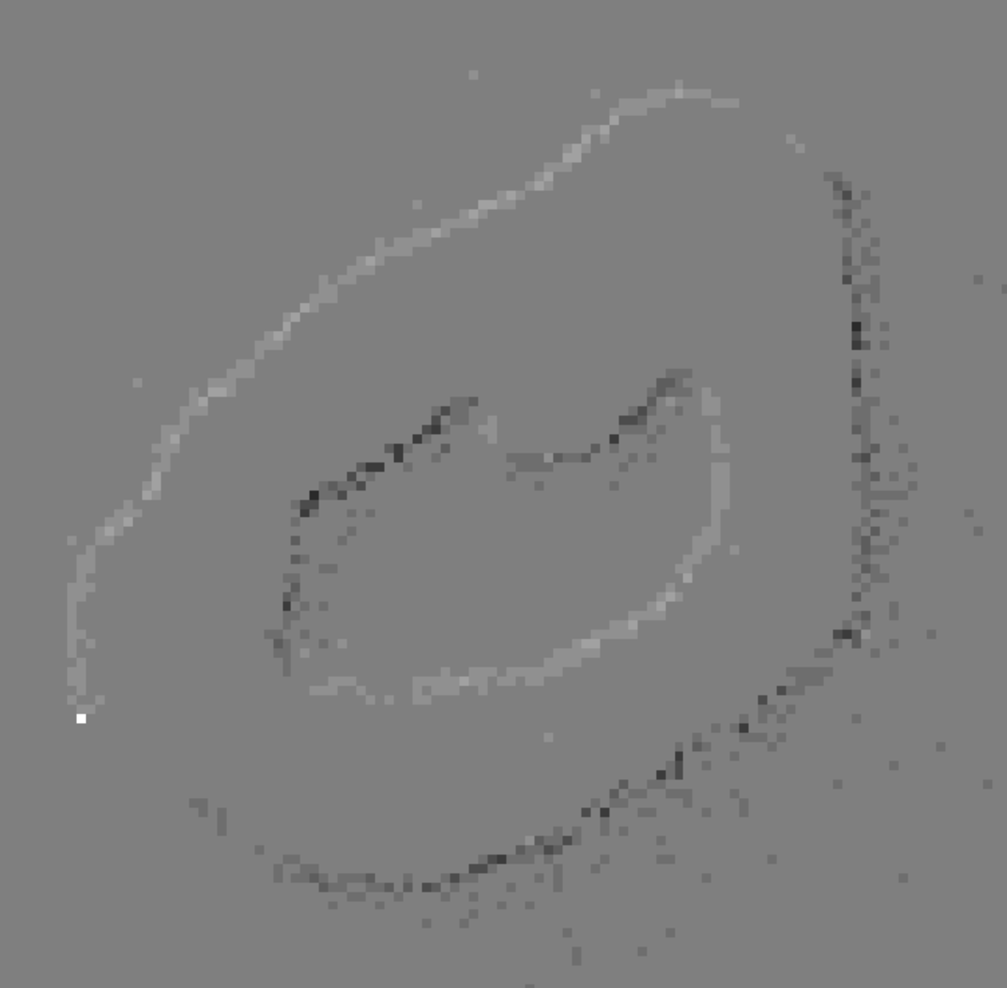
\includegraphics[width=0.22\textwidth]{images/dvs-128.pdf}
  }
  \subfloat[A snapshot of jAER playing Poissonian spike trains.]{
    \label{Fig:poisson}
    
\includegraphics[width=0.22\textwidth]{images/zero-28-2.pdf}
  }\\
  \subfloat[The raster plot of the Poissonian spike trains.]{
    \label{Fig:raster}
    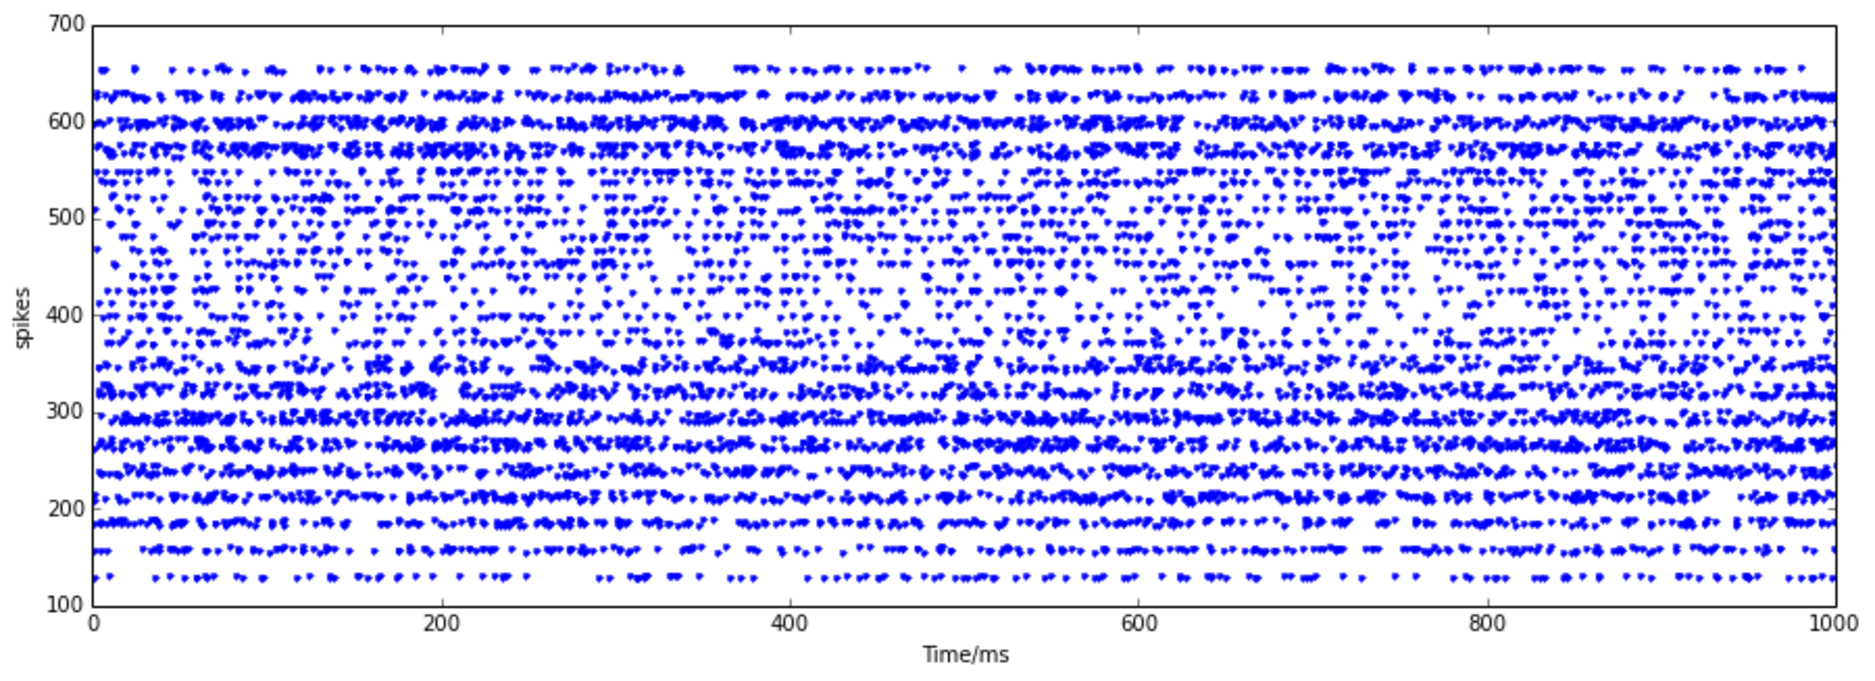
\includegraphics[width=0.48\textwidth]{images/zero.pdf}
  }
  
  \caption{Snapshots and raster plot of both the DVS recorded spikes and the Poissonian spike trains.}
  \label{fig:zero}
\end{figure}

\subsection{Data Description}	
	\subsubsection{Poissonian}
	
	In the cortex, the timing of spikes is highly irregular~[\cite{squire1998findings}].
	It can be interpreted that the inter-spike interval reflects a random process driven by the instantaneous firing rate.
	If the generation of each spike is assumed to be independent of all the other spikes, the spike train is seen as a Poisson process.
	The spiking rate can be estimated by averaging the pooled responses of the neurons.
		
	As stated above, rate coding is exclusively used in presenting images with spikes.
	The spiking rate of each neuron is in accordance with its corresponding pixel intensity.
	Instead of providing exact spike arrays, we share the Python code of generating the spikes.
	Every recognition system may require different spiking rates and various lengths of their durations.
	The generated Poissonian spikes can be in the formats of both jAER and PyNN spike source array.
	Thus, it is easy to visualise the digits and also to build spiking neural networks.
	The same digit displayed in Fig~\ref{Fig:jaer} is converted to Poissonian spike trains, see Fig~\ref{Fig:poisson}.
	The raster plot can be found in Fig~\ref{Fig:raster}, indicating the intensities of the pixels.

	
	\subsubsection{Rank-Order-Encoding}
  A different way of encoding spikes is using a rank-order code; this means
keep just the order in which those spikes were fired and disregard the exact timing. Rank-ordered spike trains have been used in vision tasks under a biological plausibility constraint, making them a viable way of image encoding for neural applications~\citep{van2001rate,sen2009evaluating,masmoudi2010novel}.

Rank-ordered encoding can be performed using an algorithm known as 
{Filter overlap Correction algorithm} or FoCal~\citep{sen2009evaluating}. It models the foveal pit region, the highest resolution area of the retina, with four ganglion cell layers that show a{centre-surround behaviour~\citep{kolb2003retina}. In order to simulate these layers, four discrete 2D convolutions are performed. The centre-surround behaviour of the ganglion cells is modelled using Differences of Gaussians~(DoG). 
\begin{equation}
\label{eq-dog}
DoG_w(x,y) = \pm\frac{1}{2\pi\sigma_{w,c}^2}e^{\frac{-(x^2 + y^2)}{2\sigma_{w,c}^2}}
\mp\frac{1}{2\pi\sigma_{w,s}^2}e^{\frac{-(x^2 + y^2)}{2\sigma_{w,s}^2}}
\end{equation}
where $\sigma_{w,c}$ and $\sigma_{w,s}$ are the standard deviation for the 
centre and surround components of the DoG at layer $w$. The signs 
will be ($-$,$+$) if the ganglion cell has an OFF-centre behaviour and 
($+$,$-$) if it has an ON-centre one. Table~\ref{tab-kernel-specs} 
describes the parameters used to compute the convolution kernels at each 
scale $w$.

\begin{table}[htb]
 \caption{Simulation parameters for ganglion cells}
  \begin{center}


  \bgroup
  \def\arraystretch{1.4}
      
  \begin{tabular}{c c c c c c}
    \begin{minipage}{0.7cm}\centering Layer \end{minipage}& 
    \begin{minipage}{0.8cm}\centering Centre \\type \end{minipage}& 
    \begin{minipage}{0.7cm} \centering Matrix width \end{minipage}&  
    \begin{minipage}{1.3cm}\centering Centre std. dev. ($\sigma_c$)\vspace*{0.1cm}\end{minipage} & 
    \begin{minipage}{1.3cm}\centering Surround std. dev. ($\sigma_s$)\vspace*{0.1cm}\end{minipage} & 
    \begin{minipage}{1.3cm}\centering Sampling resolution (cols,rows)\vspace*{0.1cm}\end{minipage} \\
    \hline
    \begin{minipage}{0.7cm}\centering 1  \end{minipage} &
    \begin{minipage}{0.8cm}\centering OFF \vspace*{0.005cm} \end{minipage}& 
    \begin{minipage}{0.7cm}\centering$3$ \end{minipage}& 
    $0.8$ & $6.7 \times \sigma_c$ &  1, 1 \\
    \begin{minipage}{0.7cm}\centering 2 \end{minipage} & 
    \begin{minipage}{0.8cm}\centering ON \vspace*{0.005cm}\end{minipage} & 
    \begin{minipage}{0.7cm}\centering $11$ \end{minipage}& 
    $1.04$ & $6.7 \times \sigma_c$ & 1, 1 \\
    \begin{minipage}{0.7cm}\centering3 \end{minipage} &
    \begin{minipage}{0.8cm}\centering OFF \vspace*{0.005cm}\end{minipage} & 
    \begin{minipage}{0.7cm}\centering $61$ \end{minipage}& 
    $8$ & $4.8 \times \sigma_c$ & 5, 3 \\
    \begin{minipage}{0.7cm}\centering 4  \end{minipage} & 
    \begin{minipage}{0.8cm}\centering ON \vspace*{0.005cm}\end{minipage} & 
    \begin{minipage}{0.7cm}\centering $243$\end{minipage} &
    $10.4$ & $4.8 \times \sigma_c$ & 5, 3 
  \end{tabular}
  \egroup
 \end{center}
  \label{tab-kernel-specs}
\end{table}

Every pixel value in the convolved images (Fig. \ref{fig-convolution-results}) 
is inversely proportional to a spike emission time (i.e. the higher the pixel value, the sooner the spike will be sent out.)

\begin{figure}[hbt]
  \centering
  \subfloat[Original image]{
    \label{sfig-rank-ordered-original}
    
\includegraphics[width=0.15\textwidth]{original_21-0}
  }
  \subfloat[Layer 1 (\textsc{off}-centre)]{
    \label{sfig-rank-ordered-midget-off}
    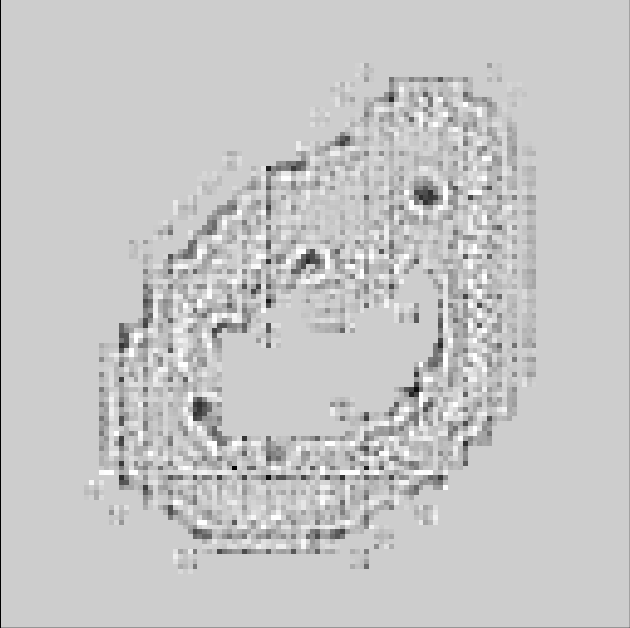
\includegraphics[width=0.15\textwidth]{filtered-21-0-layer-0}
  }
  \subfloat[Layer 2 (\textsc{on}-centre)]{
    \label{sfig-rank-ordered-midget-on}
    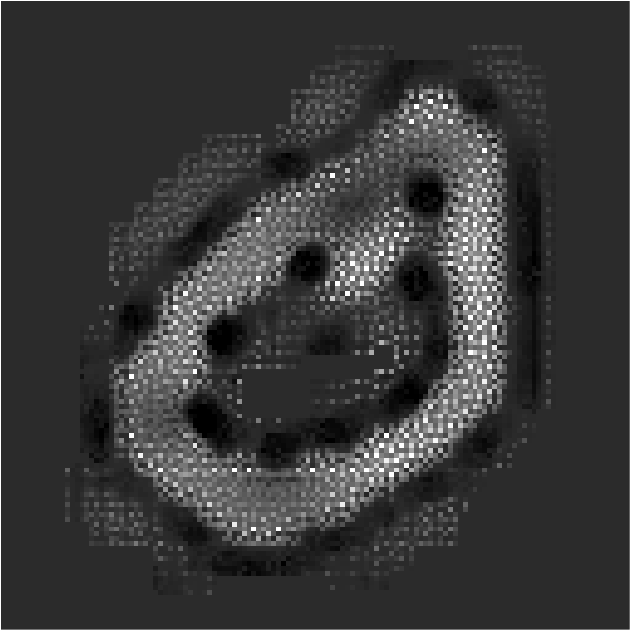
\includegraphics[width=0.15\textwidth]{filtered-21-0-layer-1}
  }\\
  \subfloat[Layer 3 (\textsc{off}-centre)]{
    \label{pic-lena-P-OFF}
    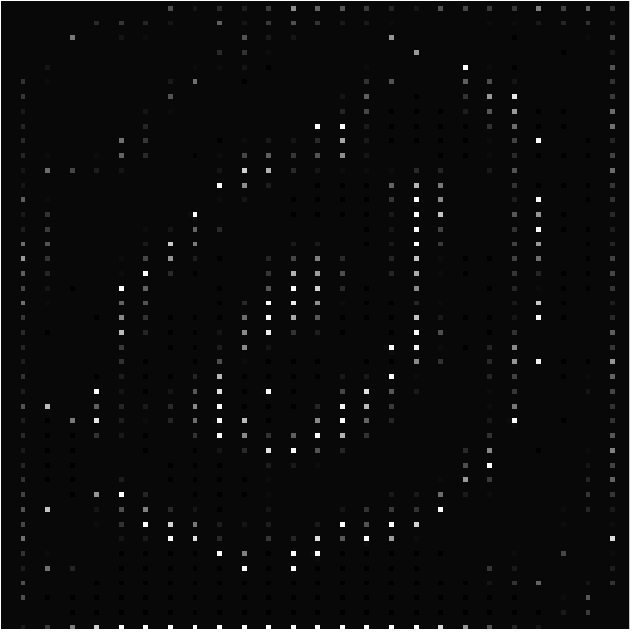
\includegraphics[width=0.15\textwidth]{filtered-21-0-layer-2}
  }
  \subfloat[Layer 4 (\textsc{on}-centre)]{
    \label{pic-lena-P-ON}
    
\includegraphics[width=0.15\textwidth]{filtered-21-0-layer-3}
  }
  \caption{Results of correcting the spikes from the simulated ganglion cell layers.}
  \label{fig-convolution-results}
\end{figure}
The algorithm also performs a redundancy correction step, it does so by 
adjusting the convolved image's pixel value according to the correlation 
between convolution kernels (Alg.~\ref{code-focal-corr}).
\begin{algorithm}[h]
  \caption{FoCal, Part 2}
  \label{code-focal-corr}
  \begin{algorithmic}
    \Procedure{Correction}{coeffs $C$, correlations $Q$}
    \State $N \leftarrow \emptyset$ \Comment{Corrected coefficients}
    \Repeat
    \State $m \leftarrow max(C)$\Comment{Obtain maximum from $C$}
    \State $M \leftarrow M \cup m$\Comment{Add maximum to $M$}
    \State $C \leftarrow C \setminus m$\Comment{Remove maximum from $C$}
    \ForAll{$ c \in C$} \Comment{Adjust all remaining $c$}
    \If{$Q(m, c) \neq 0$} \Comment{Adjust only near}
    \State $c \leftarrow c - m \times Q(m, c)$
    \EndIf
    \EndFor
    \Until{$C = \emptyset$}
    \State \textbf{return} $M$
    \EndProcedure
  \end{algorithmic}
\end{algorithm}

<<<<<<< HEAD
After the correction step, the most important information can be recovered using only the first 30\% of the spikes~\citep{sen2009evaluating}. These significant spikes are shown in Fig.~\ref{fig-raster-plot-30pc}, assuming that each spike will be generated 1~ms apart. Neurons in Layer 1 emit spikes faster and in larger quantities than any other layer, making it the most important one. Layers 2 and 3 have few spikes, this is due to the large convolution kernels used to simulate the ganglion cells. One of the main advantages of ROC is that neurons will only spike once, this can be seen particularly well in these two layers. Layers 0 and 1 encode fine details, while layers 2 and 3 result in blob like features.
\begin{figure}[hbt]
  \centering
      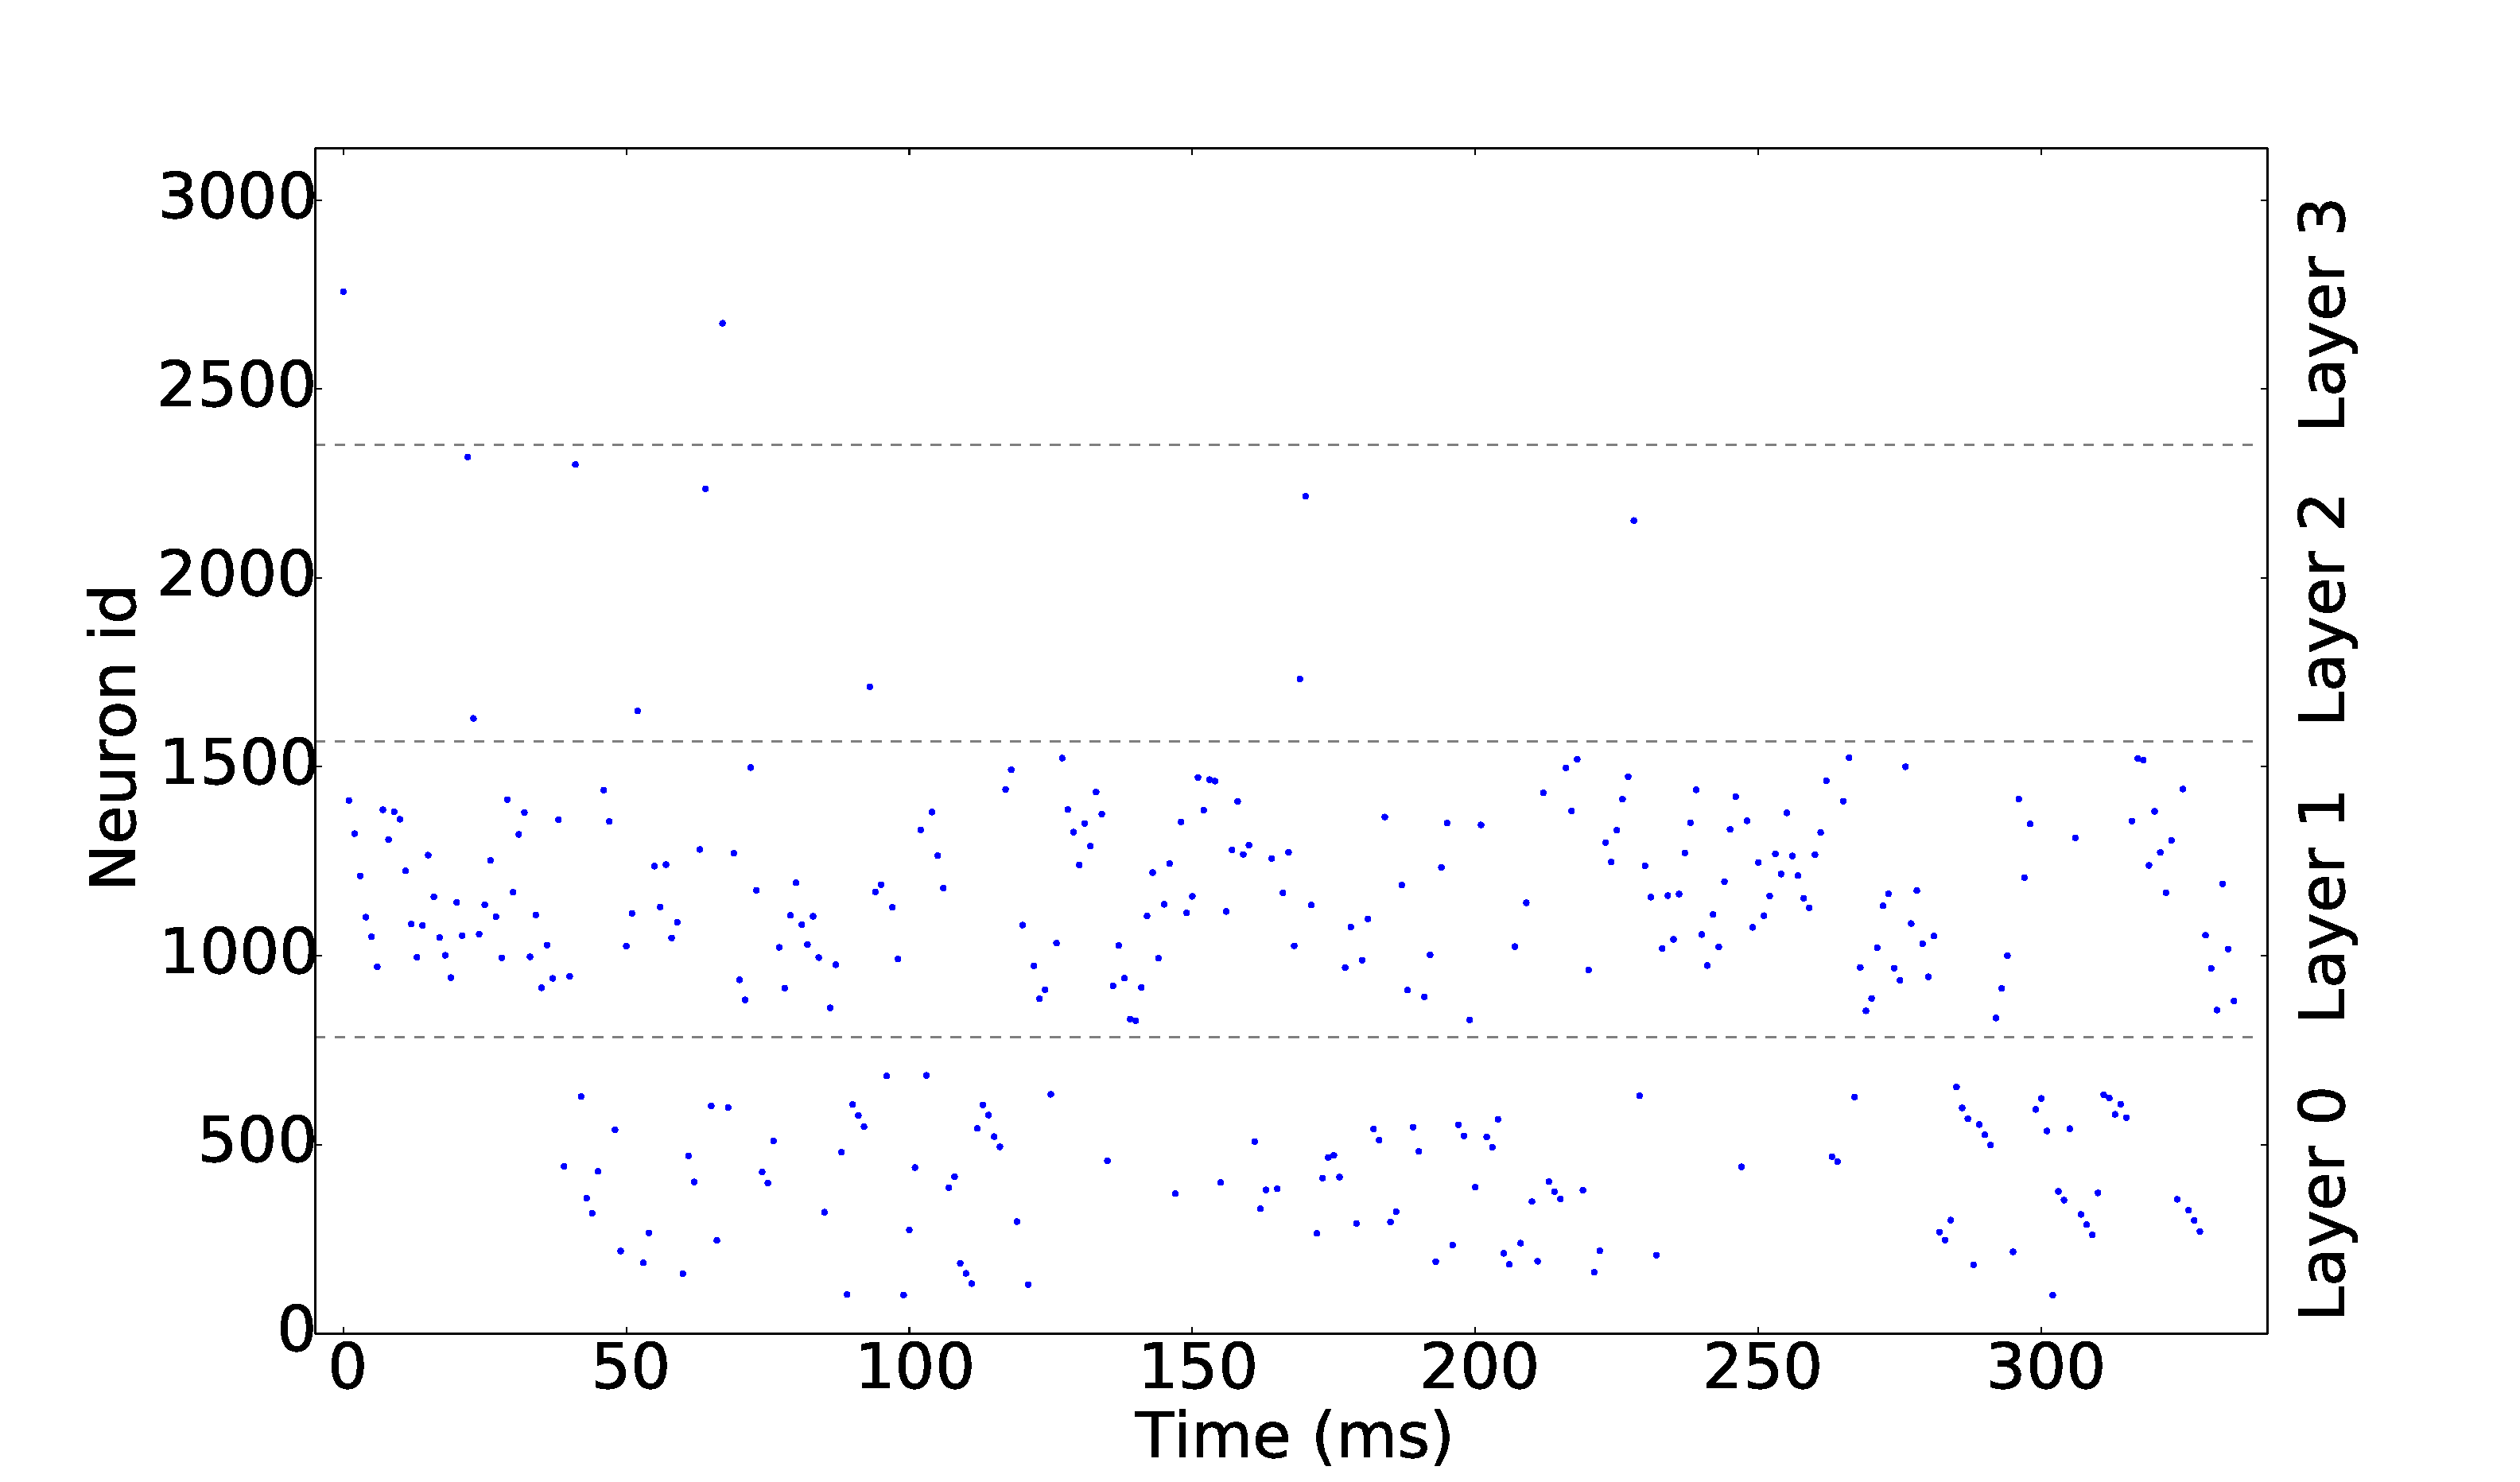
\includegraphics[width=0.475\textwidth]{raster-plot-21-0-30pc}
      \caption{First 30\% of the rank-order encoded spikes produced with FoCal.}
      \label{fig-raster-plot-30pc}
=======
After the correction step, the most important information can be recovered using only the first 30\% of the spikes~\citep{basab-model}. These significant spikes are shown in Fig.~\ref{fig-raster-plot-30pc}, assuming that each spike will be generated 1~ms apart. Neurons in Layer 1 emit spikes faster and in larger quantities than any other layer, making it the most important one. Layers 2 and 3 have few spikes, this is due to the large convolution kernels used to simulate the ganglion cells. One of the main advantages of ROC is that neurons will only spike once, this can be seen particularly well in these two layers. Layers 0 and 1 encode fine details, while layers 2 and 3 result in blob like features.

\begin{figure}[hbt]
  \centering
    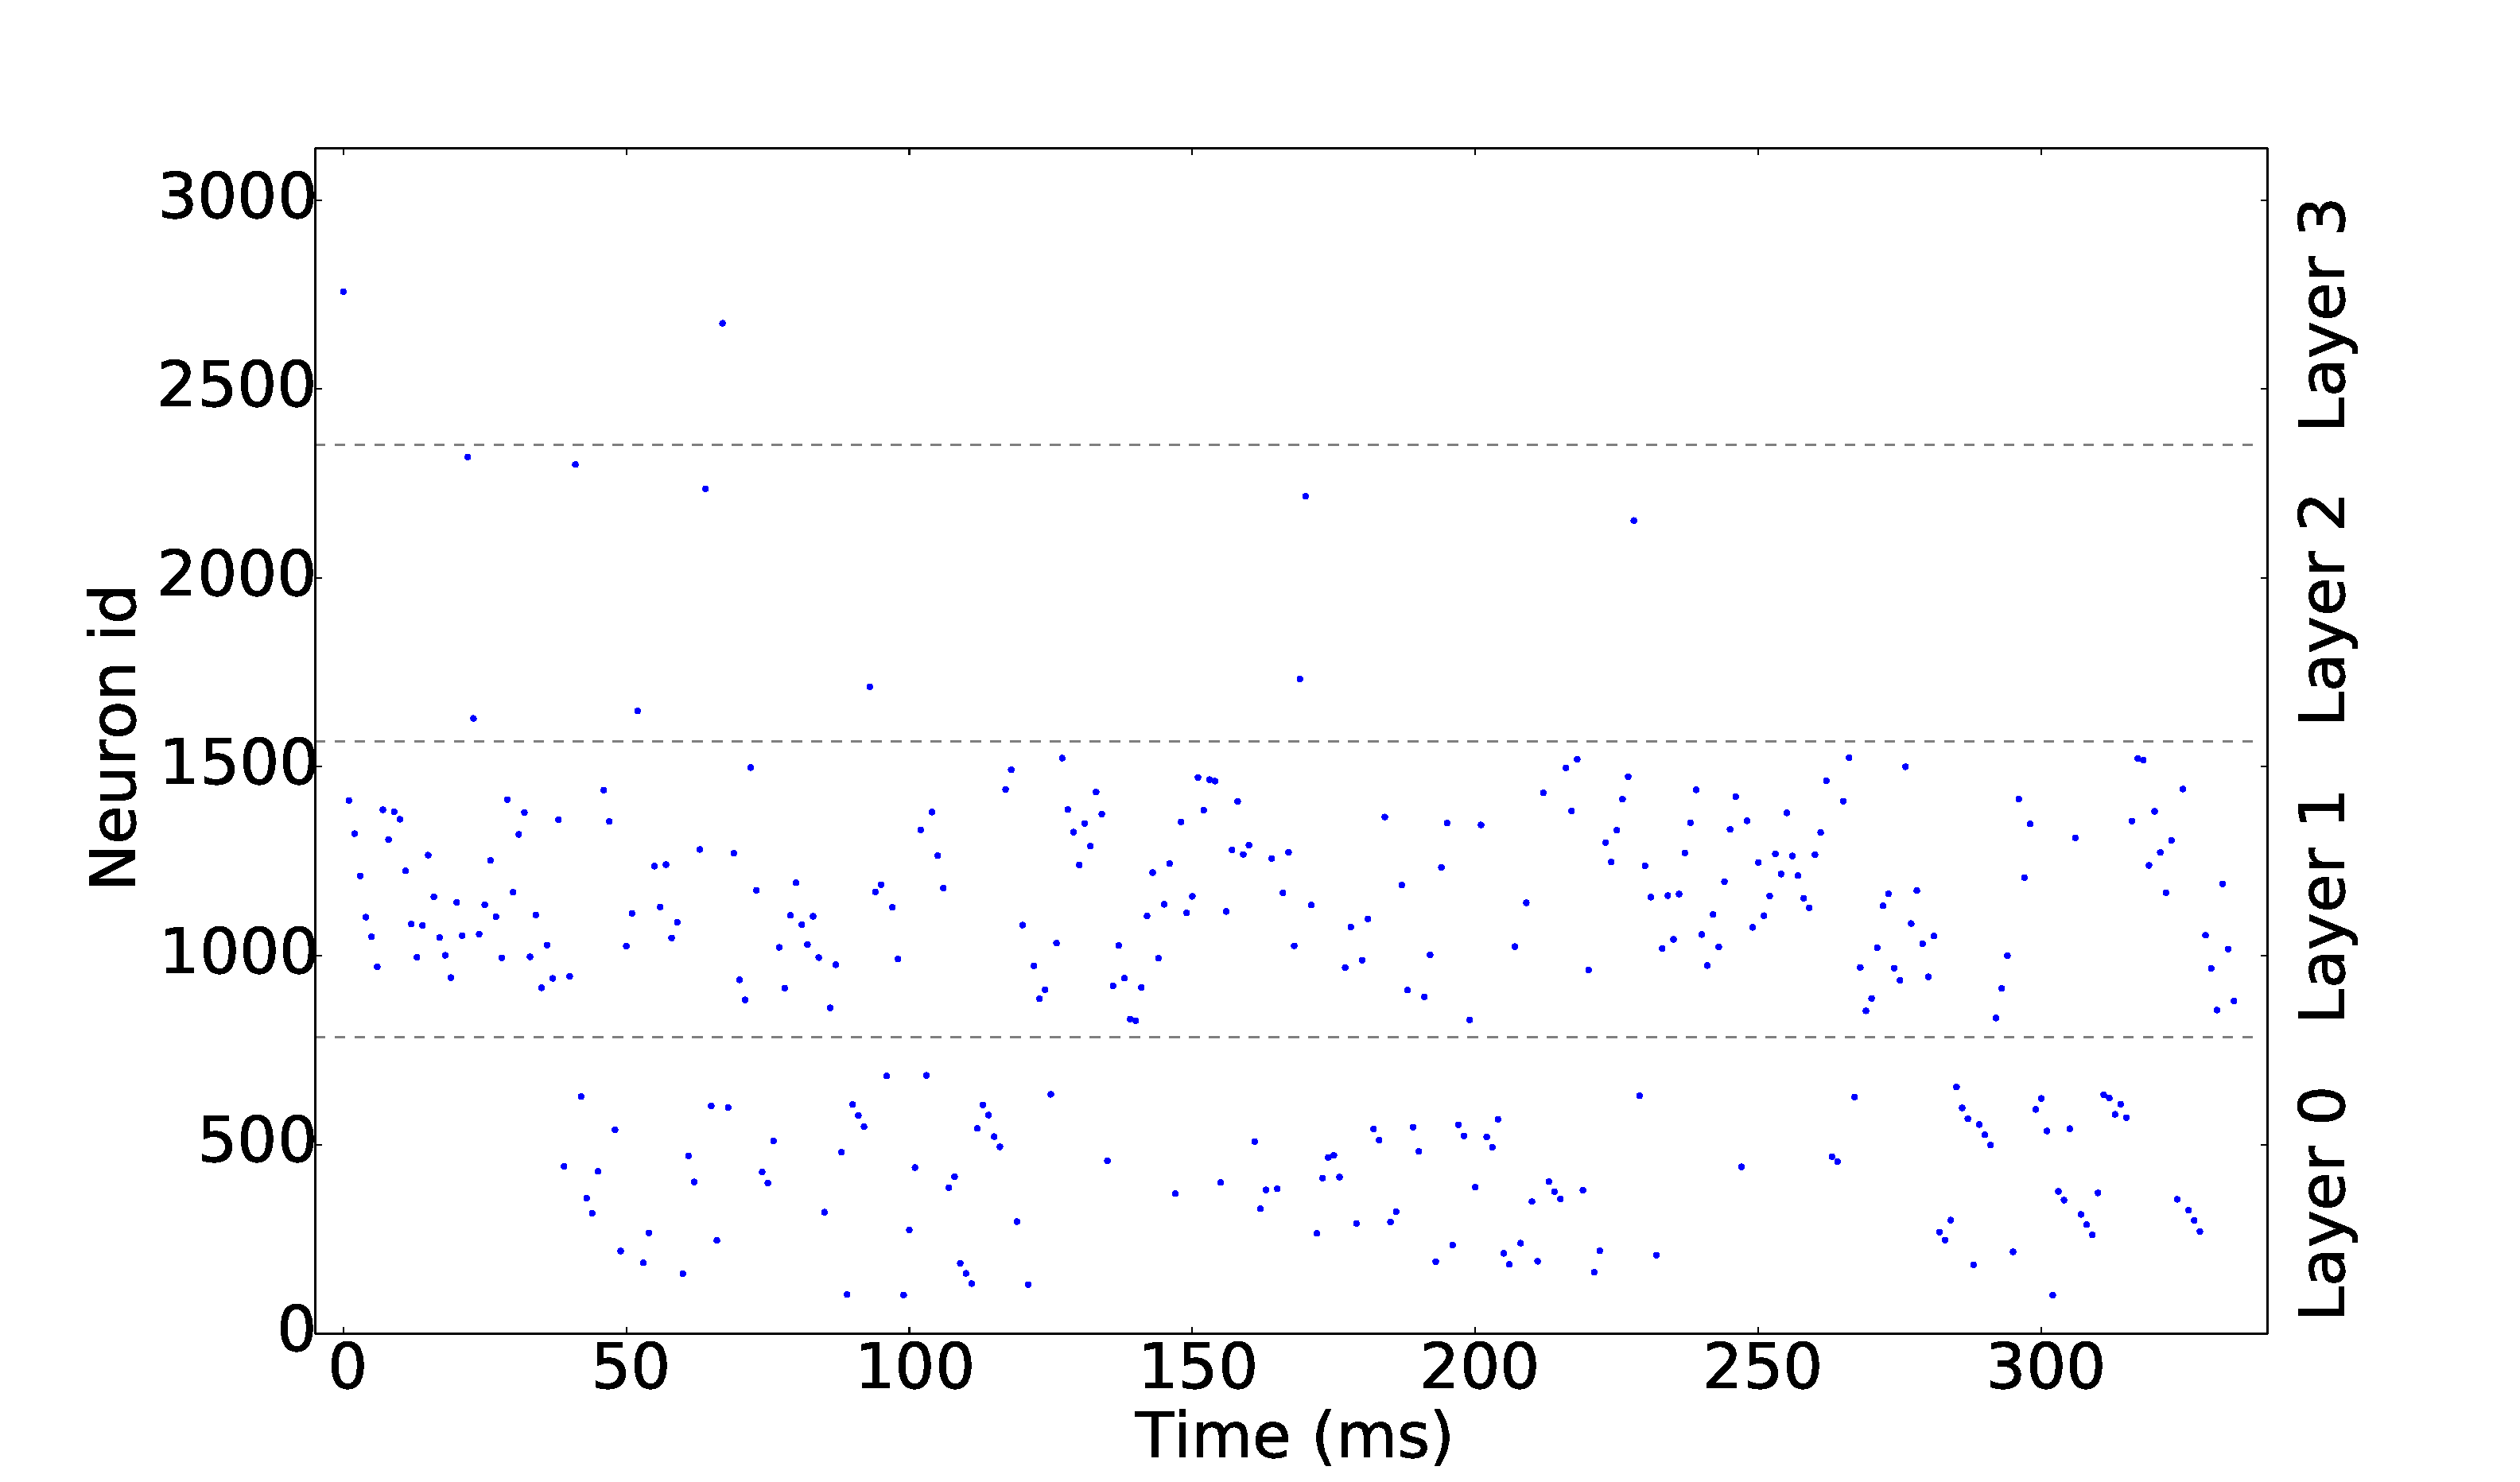
\includegraphics[width=0.475\textwidth]{raster-plot-21-0-30pc}
%    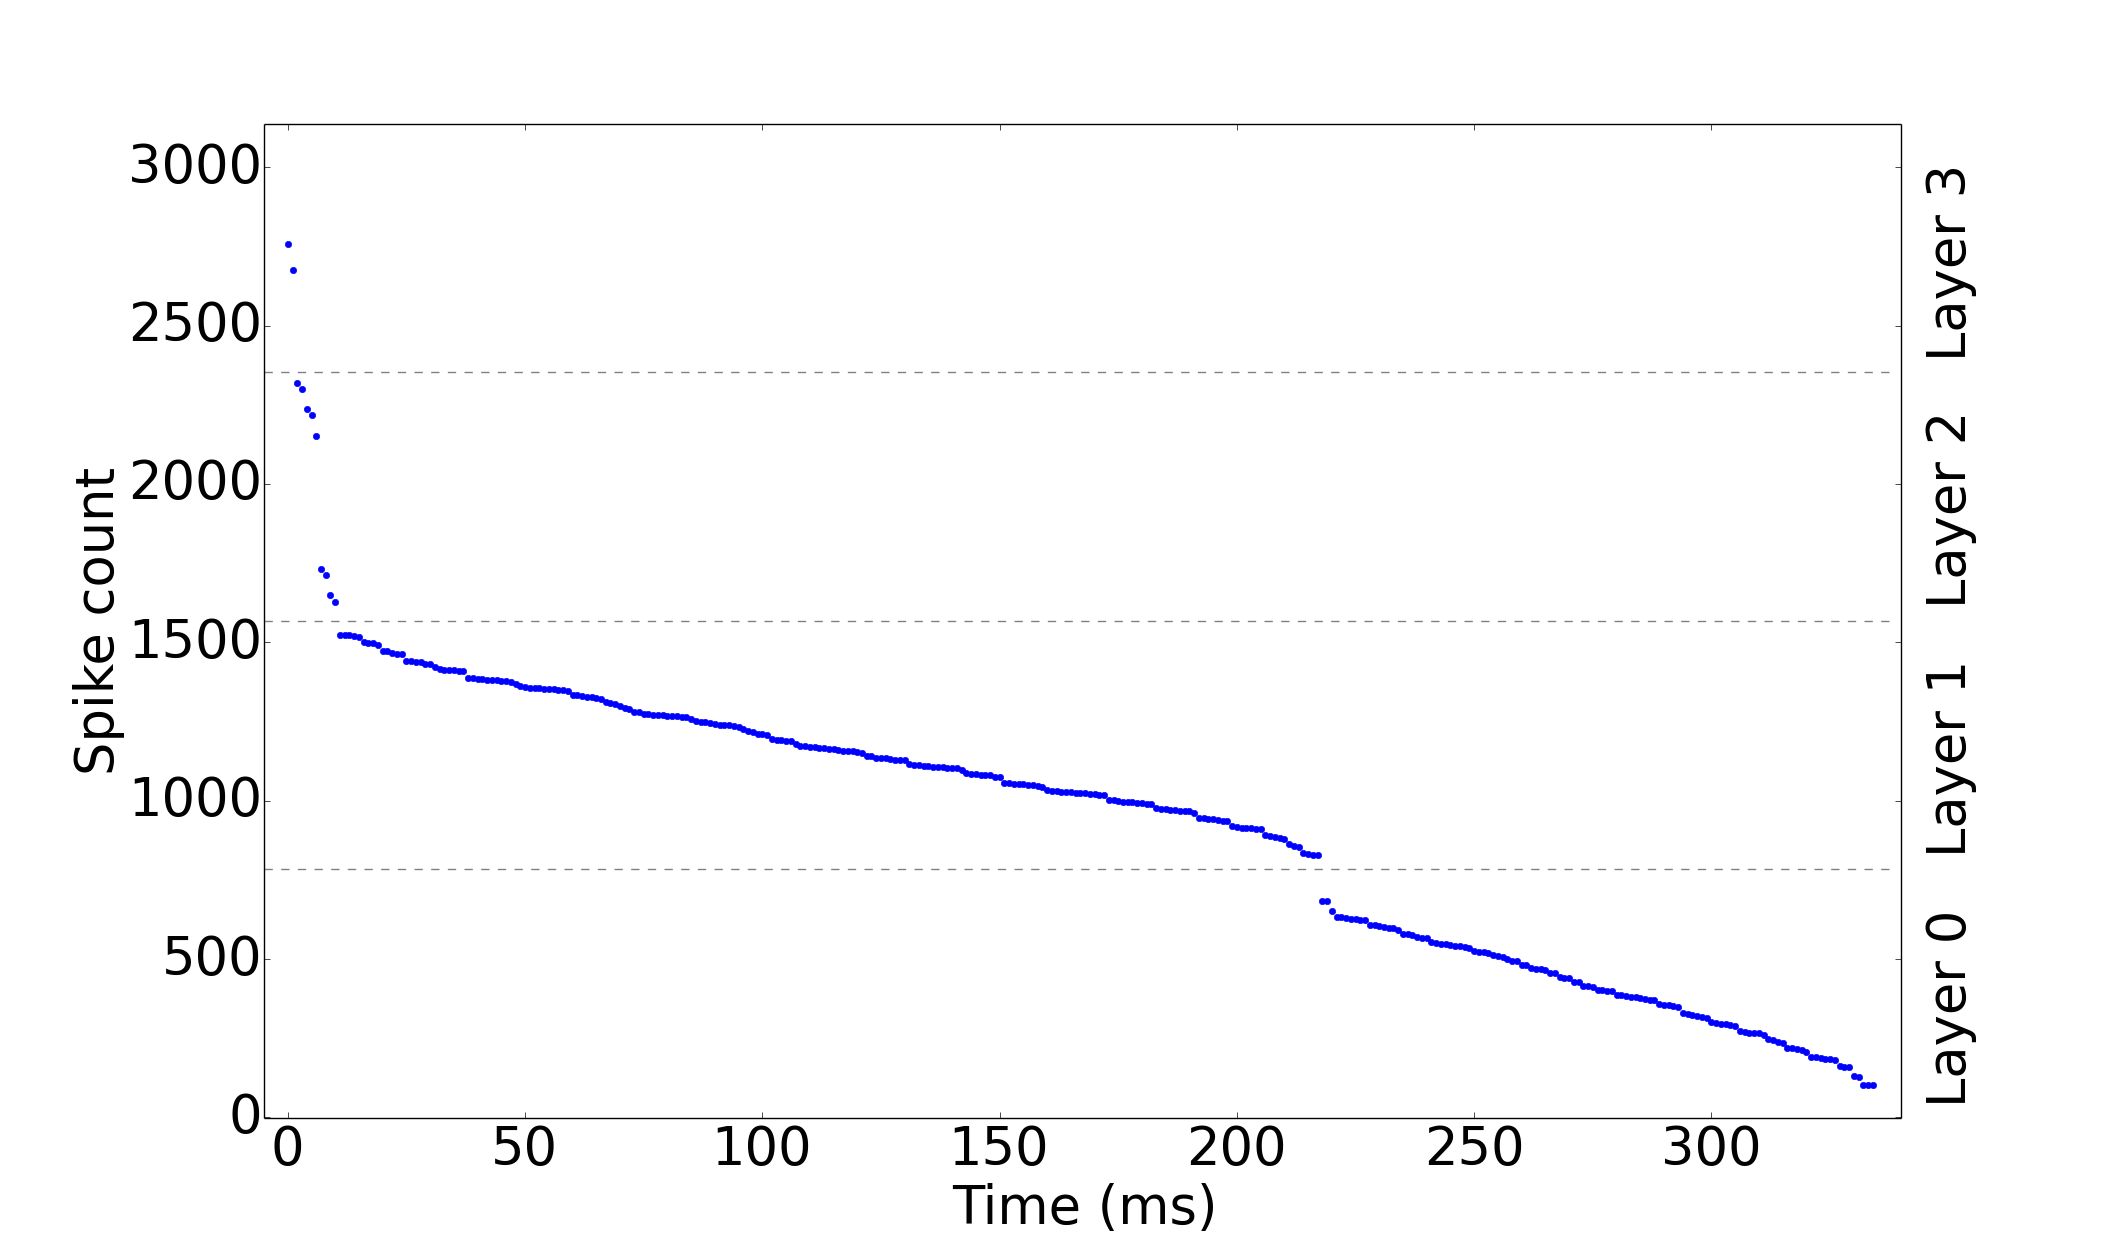
\includegraphics[width=0.475\textwidth]{sorted-raster-plot-21-0-30pc}
  \caption{First 30\% of the rank-order encoded spikes produced with FoCal.}
  \label{fig-raster-plot-30pc}
>>>>>>> 7059eb97ce659e6943f936f858bc9f8504ba0a63
\end{figure}

Figure \ref{fig-reconstruction-results} shows the reconstruction results for the two stages of the algorithm. On Fig. \ref{pic-lena-reconstructed-raw} the reconstruction was applied after the convolution, a blurry image is the result of redundancy in the spike representation. A better reconstruction can be obtained after Algorithm \ref{code-focal-corr} has been applied, the result is shown in Figure \ref{pic-lena-reconstructed-focal}.


\begin{figure}[hbt]
  \centering
  \subfloat[Original image]{
    \label{sfig-rank-ordered-original-1}
    
\includegraphics[width=0.15\textwidth]{original_21-0}
  }
  \subfloat[No correction]{
    \label{pic-lena-reconstructed-raw}
    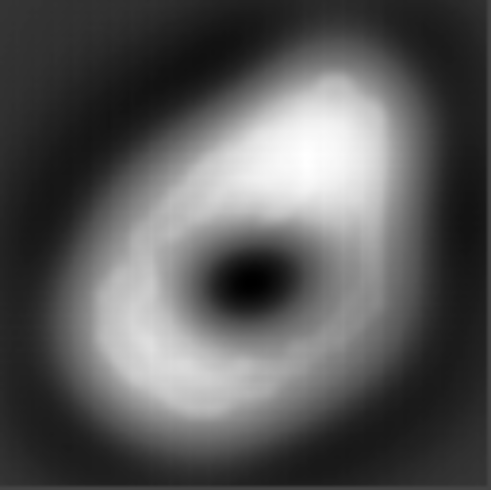
\includegraphics[width=0.15\textwidth]{reconstructed_21-0_raw}
  }
  \subfloat[FoCal]{
    \label{pic-lena-reconstructed-focal}
    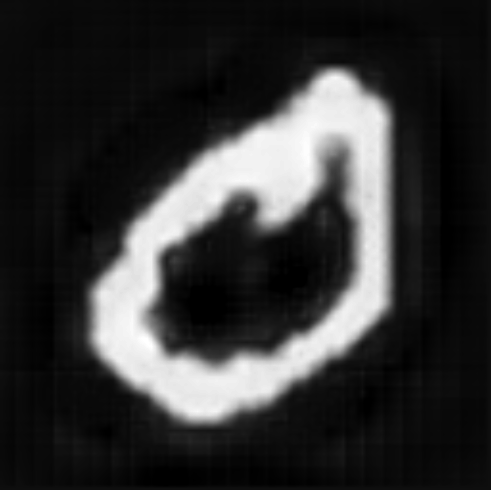
\includegraphics[width=0.15\textwidth]{reconstructed_21-0_100pc}
  }
  \caption{Reconstruction result comparison.}
  \label{fig-reconstruction-results}
\end{figure}
%Two resolutions are provided for the rank-order encoded portion of the database, the first is the original $28\times28$ one. An additional up-scaled resolution version is also provided, the images where scaled to a $128\times128$ resolution using bi-cubic interpolation, this was done to match the DVS native resolution. 

The source Python scripts to transform images to ROC spike trains, to convert the results into AER and PyNN's spike source array can be found in the dataset's website.
	\subsubsection{DVS Sensor Output with Flashing Input}
	\label{subsec_flash}
	The purposes of including the subset of DVS recorded flashing digits are to (1) promote the application of Rank-Order-Coding to DVS output; and (2) accelerate the fast on-set recognition by using just the beginning part of spike trains within less than 30~ms.
	
	Each digit and a blank image were shown alternately five times and each display lasted one second.
	The digits were displayed on a LCD monitor in front of the DVS retina~[\cite{serrano-gotarredona_128_2013}] and were placed in the centre of the visual field of the camera.
	Each recording was cut into 10 sub sections.
	Since there are two polarities of the spikes: 'ON' indicates the increase of the intensity while 'OFF' reflects the opposite, there are five 'ON' and 'OFF' flashing recordings respectively per digit.
	In Fig~\ref{fig:flash}, the bursty of the spikes is illustrated where most of the spikes occur in a 30~ms slot. 
	In total, the subset of the database contains 10$\times$60000 recordings for training and 10$\times$10000 for testing.
%	Due to the size limit of online repositories, only the third of every sequence of flashes is published.

	\begin{figure}[b!]
	  \centering
	  \subfloat[Spikes recorded in the order of neuron ID during 1s of time.]{
	  	    \label{fig:flash_all}
	  	    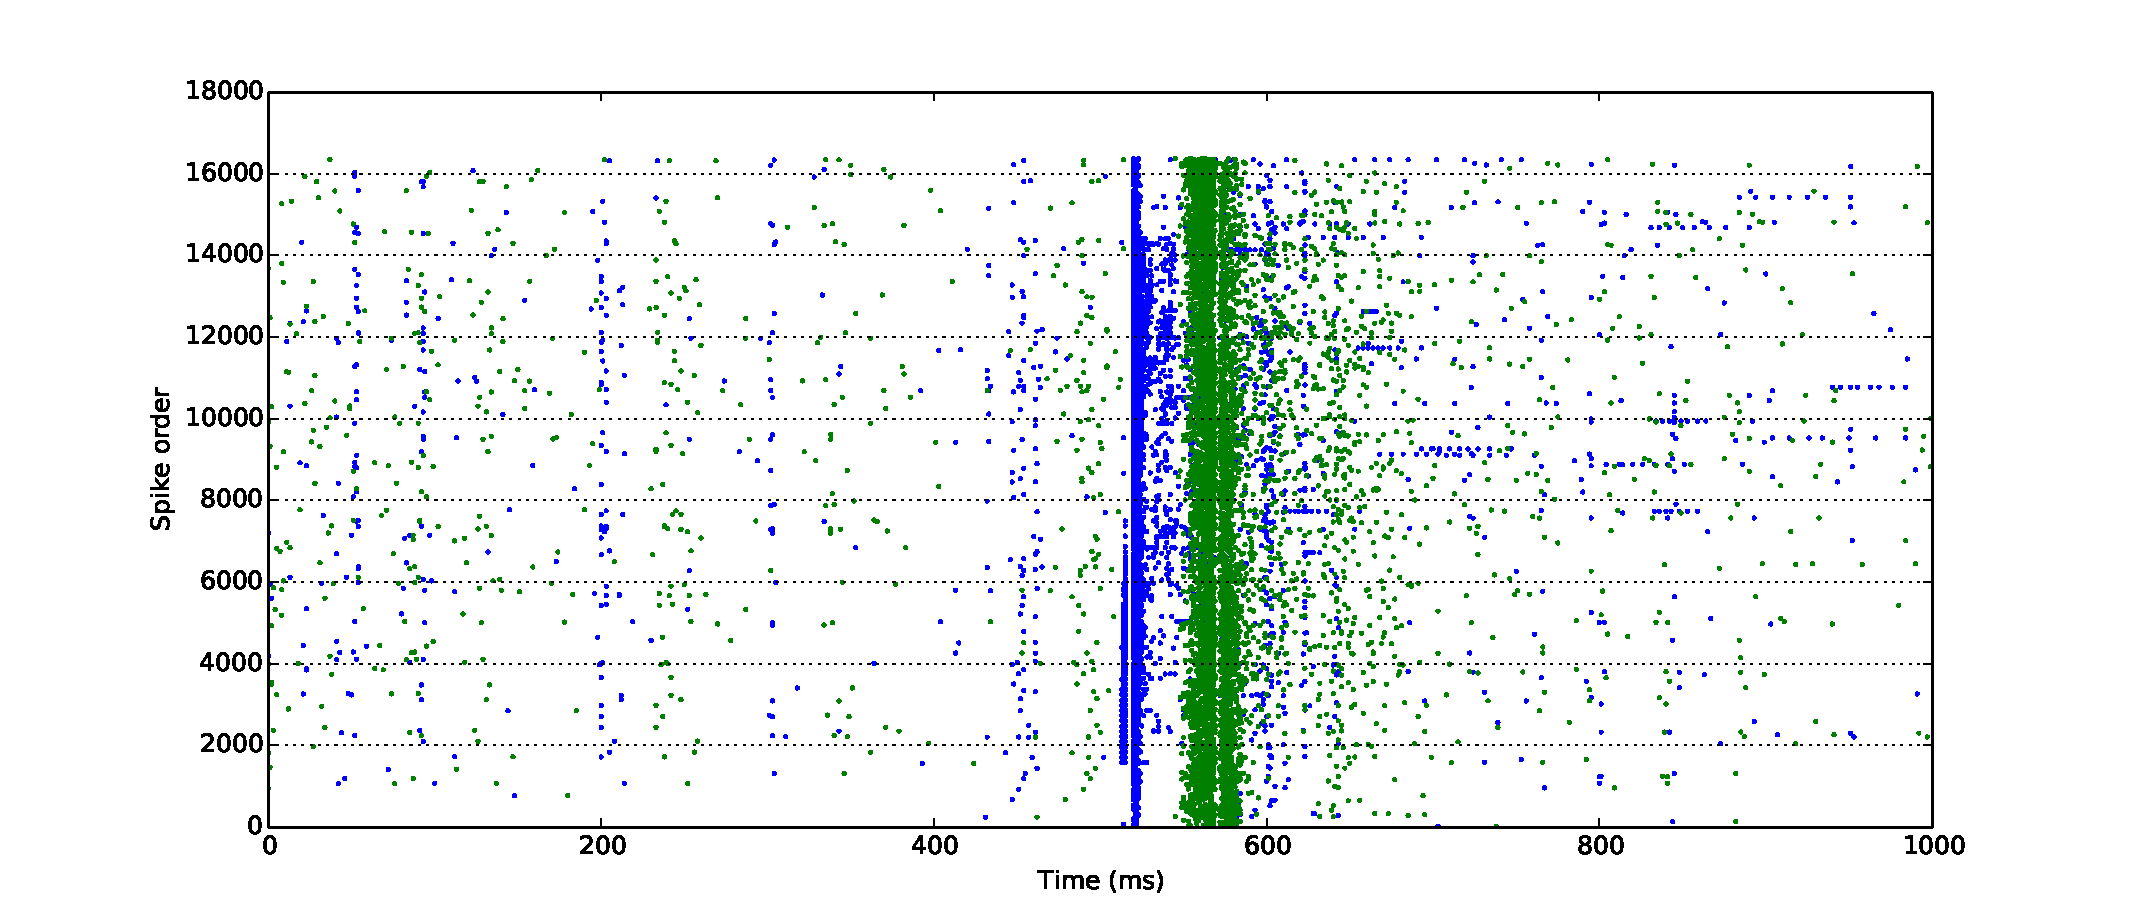
\includegraphics[width=0.48\textwidth]{flash_full.pdf}
	  	  }
	  	  \\
	  \subfloat[Spikes plotted in the sequence of appearing time during 1s of time. Bursty spikes apeer in slots less than 30~ms. ]{
	    \label{fig:flash_a}
	    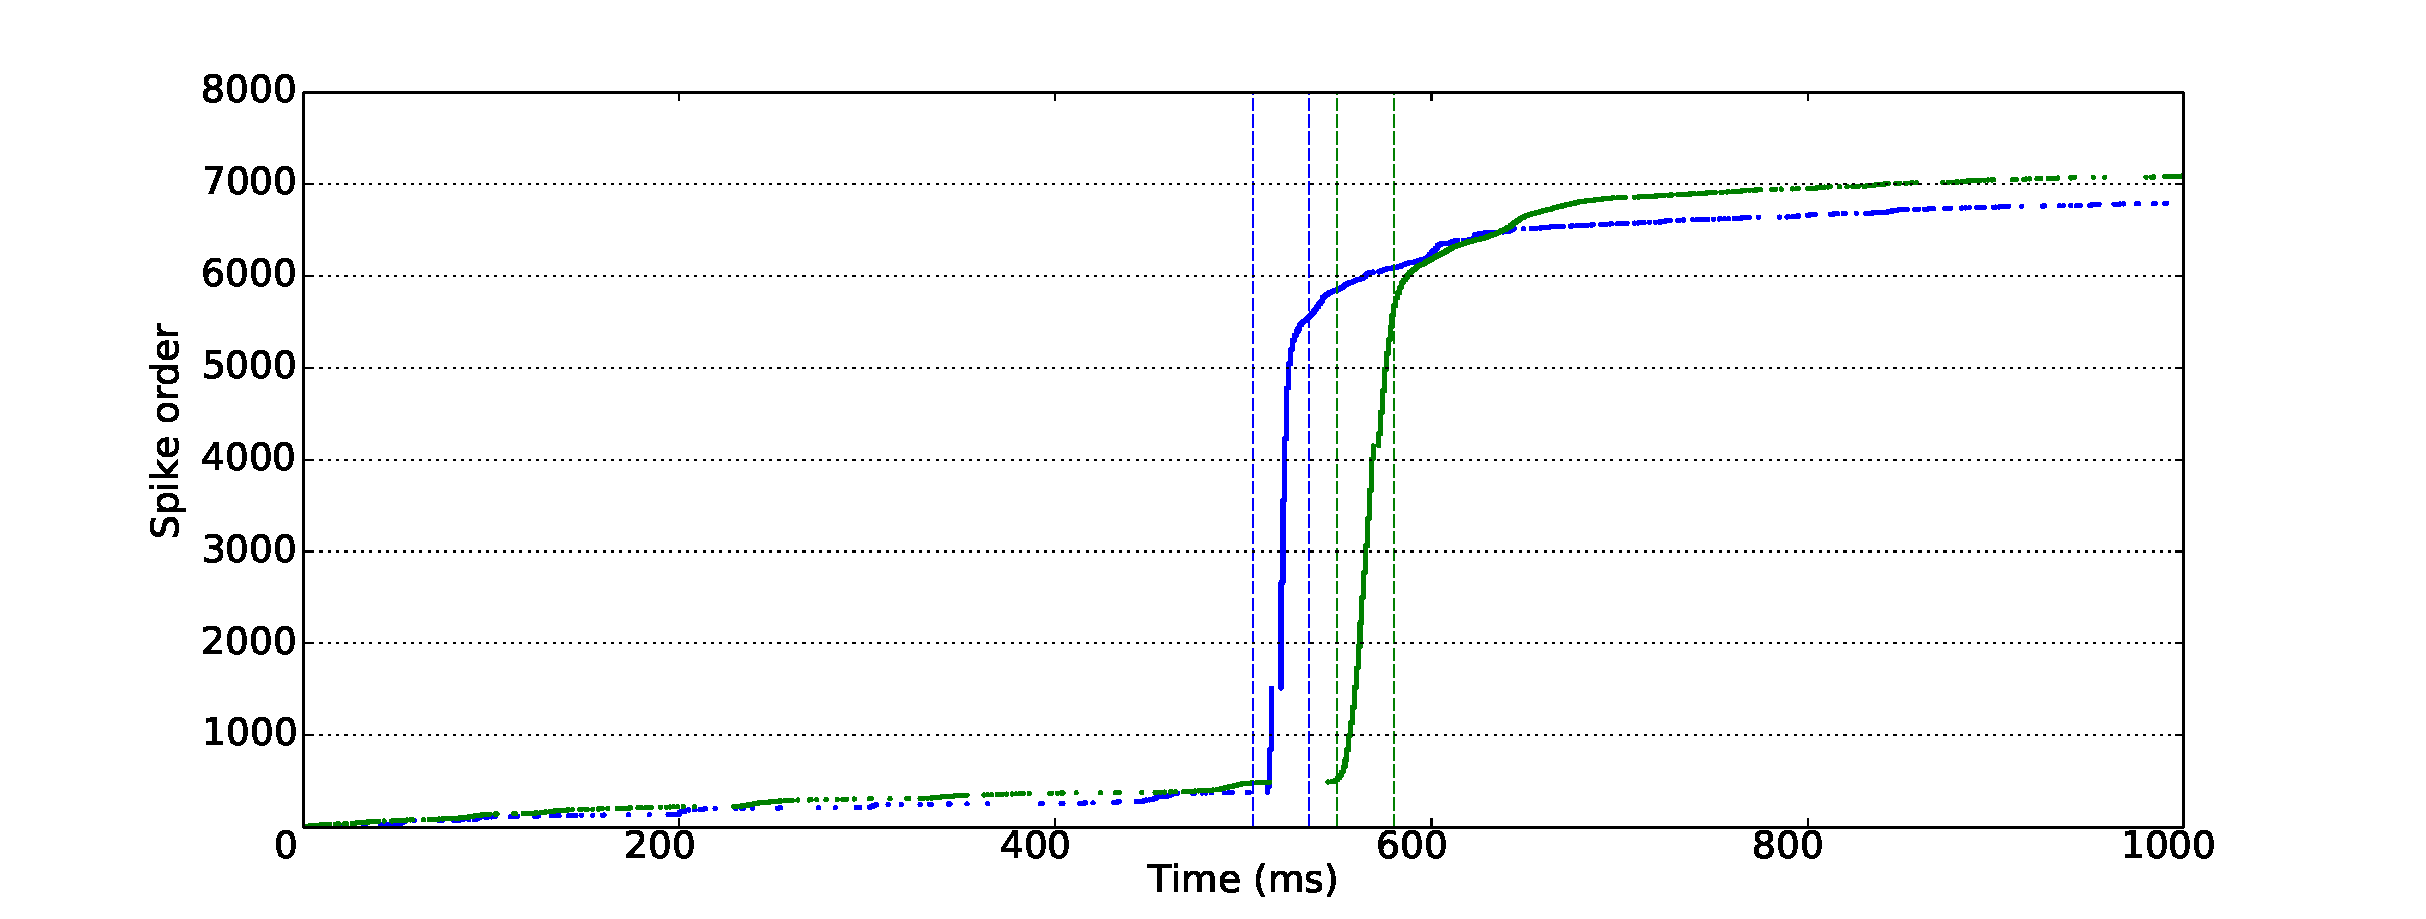
\includegraphics[width=0.48\textwidth]{flash_full_order.pdf}
	  }
%	  \\
%	  \subfloat[Bursty spikes appearing in a 30~ms slot.]{
%	  	\label{fig:flash_b}
%	  	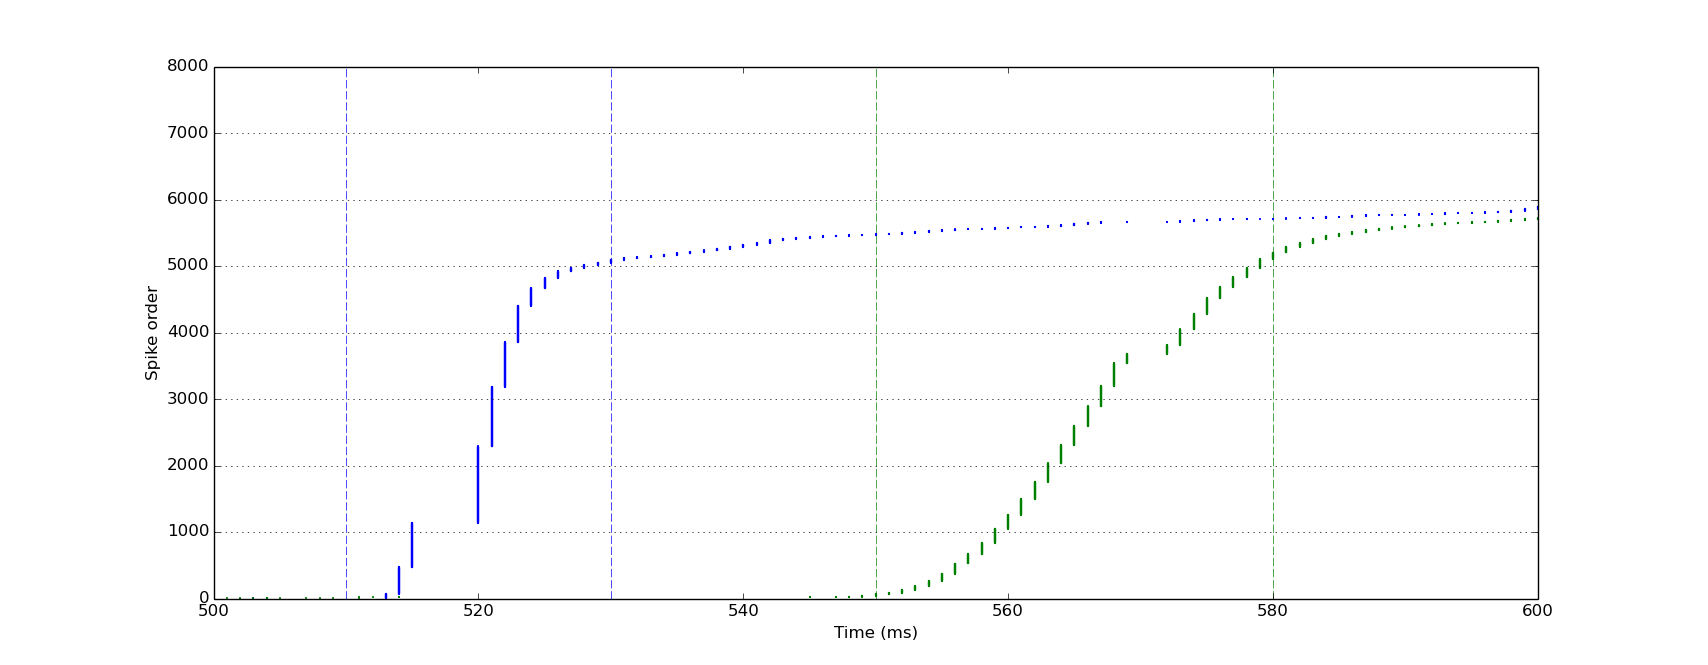
\includegraphics[width=0.48\textwidth]{flash_100.png}
%	  }

	  \caption{The bursty of spikes is illustrated where most of the spikes occur in a 30~ms slot. Blue for 'ON' events and green for 'OFF'.}
	  \label{fig:flash}
	\end{figure}
%	\subsubsection{DVS Sensor Output with Oscillating Input}
	\subsubsection{DVS Sensor Output with Moving Input}
	In order to address the problems of position- and scale- invariance, the subset of DVS recorded moving digits is presented.
	
	MNIST digits were scaled to three different sizes, by using smooth interpolation algorithms to increase their size from the original 28x28 pixel size, and displayed on the monitor with slow motion. 
	The same DVS~\cite{serrano-gotarredona_128_2013} used in Section~\ref{subsec_flash} captured the movements of the digits and generated spike trains for each pixel of its 128$\times$128 resolution.
	A total of 30,000 recordings were made: 10 characters (handwritten digits '0' to '9'), at 3 different scales, 1000 different handwritten samples for each.
	The subset is available at the website\footnote {http://imse-cnm.csic.es/caviar/MNIST\_DVS}.
	
\section{Performance Evaluation}
\label{sec:eval}

A crucial part of research is reporting results and comparing achievements with other state-of-the-art work. Unfortunately there is no standard way of fulfilling those tasks, which, sometimes, leads to confusion for the reader. We feel that the neuroscience community would benefit from a common ground for NN characteristics.

As neuromorphic hardware is more commonly used in research, larger and more complex NN models could be used. Additionally, performance of the network may be influenced by the chosen development platform. We would like to assist with the following considerations when facing these impending changes.
\begin{table*}[hbt!]
  \caption{Hardware independent comparison}
  \begin{center}
    \bgroup
    \def\arraystretch{1.5}
    \begin{tabular}{ l  c c c c }
      $ $ &
      \begin{mycell}{1.9cm}Preprocessing\end{mycell} & 
      \begin{mycell}{3.5cm} Network\end{mycell} & 
      \begin{mycell}{3.5cm} Training \end{mycell} & 
      \begin{mycell}{3.5cm} Recognition \end{mycell} \\
%      \cline{3-5}
%       & 
%       & 
%      \begin{mycell}{3.5cm}Topology, neuron and synapse models, \\extra classifier  \end{mycell} &
%      \begin{mycell}{3.5cm}Methodology, simulation time, sample repetition \end{mycell} & 
%      \begin{mycell}{3.5cm}Events/$s$, time/sample, response time, accuracy\end{mycell} \\
      \hline
%contents
      \begin{mycell}{2.5cm} \cite{Diehl2015fast}\end{mycell}  & 
      \centering None & 
      \begin{mycell}{3.5cm} ConvNet or \\FCnet, LIF neurons \end{mycell}& 
      \begin{mycell}{3.5cm} Pre-trained with ReLU, weight normalization \end{mycell}&  
      \begin{mycell}{3.5cm} 99.1\% (ConvNet), \\ 98.6\% (FCnet);\\
        Sim. time [0.5$s$, 5$s$] \end{mycell}\\
      %
      \begin{mycell}{2.5cm} \cite{brader2007learning} \end{mycell} & 
      \begin{mycell}{1.9cm} None \end{mycell} & % preprocessing
      \begin{mycell}{3.5cm} Two layer, LIF neurons\end{mycell}&  % network
      \begin{mycell}{3.5cm} Semi-supervised, STDP, calcium LTP/LTD\end{mycell}&  % training
      \begin{mycell}{3.5cm} 96.5\% \\ (2.2\% non-class, \\1.3\% wrong-class)\end{mycell} \\% recognition
      %
      \begin{mycell}{2.5cm} \cite{Diehl2015unsupervised} \end{mycell} & 
       \centering None &
       \begin{mycell}{3.5cm} Two layers, LIF neurons, inhibitory feedback  \end{mycell}& 
       \begin{mycell}{3.5cm} Unsupervised, exp. STDP, %adaptive membrane potential, 
         $150ms$ silence between samples \end{mycell} & 
       \begin{mycell}{3.5cm} 95\% \end{mycell}\\
      %
      \begin{mycell}{2.5cm} \cite{Stromatias2015scalable} \\ This paper \end{mycell} & 
      \begin{mycell}{1.9cm} None \end{mycell} & % preprocessing
      \begin{mycell}{3.5cm} Four layer RBM, \\ LIF neurons \end{mycell}&  % network
      \begin{mycell}{3.5cm} Pre-trained, unsupervised \end{mycell}&  % training
      \begin{mycell}{3.5cm} 95.1\% \end{mycell} \\% recognition
      %
      \begin{mycell}{2.5cm} \cite{neftci2013event} \end{mycell} & 
      \begin{mycell}{1.9cm} Thresholding\end{mycell} & % preprocessing
      \begin{mycell}{3.5cm} Two layer RBM, \\ LIF neurons \end{mycell}&  % network
      \begin{mycell}{3.5cm} Event-driven contrastive divergence, supervised \end{mycell}&  % training
      \begin{mycell}{3.5cm} 91.9\% \end{mycell} \\% recognition
      %
      \begin{mycell}{2.5cm} \cite{beyeler2013categorization} \end{mycell} & 
      \begin{mycell}{1.9cm} None \end{mycell} & % preprocessing
      \begin{mycell}{3.5cm} V1 (edge), \\V4 (orientation),\\ and competitive decision, Izhikevich neurons\end{mycell}&  % network
      \begin{mycell}{3.5cm} Semi-supervised, STDP, \\ calcium LTP/LTD \end{mycell} &  % training
      \begin{mycell}{3.5cm} 91.6\% \\ (8.3 \% non-class, \\ 0.1\% wrong-class) \end{mycell} \\% recognition
      %
      \begin{mycell}{2.5cm} \cite{zhao_feedforward_2014}\end{mycell}  & 
      \begin{mycell}{1.9cm} Thresholding or DVS \end{mycell}& % preprocessing 
      \begin{mycell}{3.5cm} Simple (Gabor), \\Complex (MAX) \\and Tempotron  \end{mycell}& % network
      \begin{mycell}{3.5cm} Tempotron, supervised \end{mycell}& % training
      \begin{mycell}{3.5cm} 91.3\% (threshold) \\ $88.1\% $ (DVS)\end{mycell}\\ % recognition
      \begin{mycell}{2.5cm} This paper \end{mycell}  & 
      \begin{mycell}{1.9cm}  K-means clusters \end{mycell}& % preprocessing 
      \begin{mycell}{3.5cm} FC decision layer, \\ LIF neurons \end{mycell}& % network
      \begin{mycell}{3.5cm} Supervised STDP \end{mycell}& % training
      \begin{mycell}{3.5cm} 90.0\% \end{mycell}\\ % recognition
    \end{tabular}
    \egroup
  \end{center}
  \label{tb:software_comparison}
\end{table*}

\subsection{Hardware-Independent}
\label{subsec:model}
As we are proposing spike based data-sets or a methodology to produce them, it's desirable that the users specify whether they added any further processing either to images or spikes~[\cite{best-practice-nn-img}]. This is important, for example, if we want to use a modified set to test noisy inputs.

A description of the network is most welcome, as it is the basis for the overall performance. Furthermore, sharing this designs may inspire fellow scientists to create new structures that, might take a new point of view to the problem, generating a positive feedback loop where everybody wins. We believe the \emph{network description} should include some of the following elements:
%{ 
%  \setlength{\leftmargini}{0.3cm}
%  \begin{itemize}
    %\item[] \hspace*{-0.3cm} 
    \textit{Topology}, % \newline
    which includes the number of neurons, how where they arranged and the interaction between them. 
    %  What are the elements of the network (layers, populations)?
    %  How are the different elements of the network arranged? Does the arrangement have any physical or biological interpretation? What are the interactions between them? What was the intuition behind this particular topology?
    %\item[] \hspace*{-0.3cm} 
    Additional details on the \textit{neuron model}, %\newline
    like the activation function and any particulars of the implementation.
    %Does the model have a I\&F behaviour? What particular model was used?
    %\item[] \hspace*{-0.3cm} 
    The \textit{synaptic plasticity model} %\newline
    is key for learning in the network, so the report should include a description of its characteristics (e.g. short-term and/or long-term).
    %In terms of synapse, what was the  used? Does the network support short-term and/or long-term plasticity?
    %\item[] \hspace*{-0.3cm} 
    %\textit{Extra classifier}. %\newline
      Some research make use of \emph{extra non-neural classifiers}, sometimes to aid the design others to enhance the output of the NN. Any particulars on this subject are greatly appreciated.
  %\item[]
%  \end{itemize}
%}


An important distinction to make, we think, is the nature of the \emph{training} procedure. A clear distinction has always been made between supervised, semi-supervised and unsupervised learning. Other specifications are the simulation time each sample is presented to the network, whether repeating samples was necessary and if they were presented continuously or with some ``silence'' was introduced between samples. Most works use adaptations to learning rules, details on the particular modifications are highly desired. Particulars on any additional weight-changing procedures used in the simulation are always welcome.

%Also, details on the particulars of the applied learning rule (e.g. STDP, BCM), was it modified somehow?

In the testing phase, the characteristics of the \emph{recognition} should include details on the way the samples where presented (e.g. events per simulation time unit, simulation time per sample). An interesting characteristic to report, particularly for deep networks, is the response time, although this might not be measured as often. A commonly reported characteristic is the accuracy of the network, perhaps adding remarks on how these scores were obtained could help to unify criteria and ease comparison.

%Most classification papers report a percentage of accuracy that gives the reader a measure of the correct classifications~[\cite{dietterich1998approximate}]. Some times it might be desirable, for a better understanding of the paper, that a distinction between ambiguous, outliers and incorrect classes is made~[\cite{liu2002performance}]. A very useful piece of information is clear citation of the base-line source, which is almost always there but lost in a sea of references.

%Should we report also incorrect or ambiguous? Could some ``correct'' be masking ambiguous? Were the ambiguous due to noise? Was the noise added on purpose? 


%Traditionally, neural network training has been done using rate-based encoding. As new theories emerge, a


%One the biggest distinctions on learning procedures is whether they were done using some \emph{supervision} or not; making this distinction clear is vastly appreciated. On supervised learning, the label of the data influences to establish categories and connection weights. Unsupervised learning has fewer constraints when it comes to class creation but might be tougher to get right. 

%A number of different classes are expected, this quantity might give an insight onto the network topology and dynamics. A description of the methods used to generate and populate the classes is very helpful for the reader. (e.g. Did we use a statistical measure? Was it a combination of NN with some other algorithms?)




\subsection{[Evangelos Stromatias] Hardware-Specific}
\label{subsec:hw}
\begin{table*}[thb!]
  \caption{Hardware dependent comparison}
  \begin{center}
      \bgroup
      \def\arraystretch{1.4}
    \begin{tabular}{l | c c c c c c c c c}
      $ $ & 
       \begin{minipage}{2.0cm}\centering System \end{minipage} & 
%       \begin{minipage}{1.3cm}\centering Simulation type \end{minipage} & 
       \begin{minipage}{2.0cm}\centering Scalable \end{minipage} & 
       \begin{minipage}{2.0cm}\centering Programmable \end{minipage} & 
%       \begin{minipage}{1cm}\centering Axonal delays \end{minipage} & 
%       \begin{minipage}{1cm}\centering Synaptic model \end{minipage} & 
       \begin{minipage}{2.0cm}\centering Precision \end{minipage} &  
%       \begin{minipage}{1.2cm}\centering Synaptic precision \end{minipage} & 
%       \begin{minipage}{1.2cm}\centering Energy per SE \end{minipage} & 
%       \begin{minipage}{1.4cm}\centering Synaptic ops per Watt \end{minipage} & 
       \begin{minipage}{2.0cm}\centering Simulation Time \end{minipage} & 
       \begin{minipage}{2.0cm}\centering Energy Use \end{minipage} & 
%       \begin{minipage}{1.7cm}\centering Programming front-end \end{minipage}  
	   \\
       \hline
       % contents!
       \begin{minipage}{1.8cm}\centering \vspace*{0.1cm} SpiNNaker \citep{strometal} \end{minipage} & \begin{minipage}{2.0cm}\centering Digital \\ Event-driven \end{minipage} & Yes & \begin{minipage}{2.0cm}\centering Neuron/Synapse \\ Axonal delay \\ Learning rule \end{minipage}  & Programmable & \begin{minipage}{2.0cm}\centering Real-time \\ Flexible time resolution \end{minipage}  &\begin{minipage}{2.5cm}\centering 8~nJ/SE \\54.27 MSops/W \end{minipage} \\
       \begin{minipage}{1.8cm}\centering \vspace*{0.1cm} TrueNorth \citep{Merolla08082014}\end{minipage} & Digital& & & & & 46 GSops/W \\
       \begin{minipage}{1.8cm}\centering \vspace*{0.1cm} Neurogrid \citep{Benjamin_etal14}\end{minipage} &Mixed-mode& & & & & & & & \\
       \begin{minipage}{1.8cm}\centering \vspace*{0.1cm} HI-CANN \citep{Schemmel_etal10}  \end{minipage} & Mixed-mode & & & & & & \\
       \begin{minipage}{1.8cm}\centering \vspace*{0.1cm} iAER-IFAT \citep{gert}\end{minipage} &Mixed-mode & & & & & & 
       
    \end{tabular}
    \egroup
  \end{center}
  \label{tb:hardware_comparison}
\end{table*}

Depending on how neurons, synapses and spike transmission are implemented neuromorphic systems can be categorised as either analogue, digital, or mixed-mode analogue/digital VLSI circuits. Analogue implementations exploit the sub-threshold transistor dynamics to emulate neurons and synapses directly on hardware \citep{giacom} and are more energy-efficient while requiring less area than their digital counterparts \citep{temamanalogdigital}. However, the behaviour of analogue circuits is largely determined during the fabrication process due to transistor mismatch \citep{giacom,analoguemismatch,bernabeDACsynapses}, while their wiring densities render them impractical for large-scale systems. The majority of mixed-mode analogue/digital neuromorphic platforms, such as High Input Count Analog Neural Network (HI-CANN) \citep{Schemmel_etal10}, Neurogrid \citep{Benjamin_etal14}, HiAER-IFAT \citep{gert}, use analogue circuits to emulate neurons and digital packet-based technology to communicate spikes as AER events. This enables reconfigurable connectivity patterns, while the time of spikes is expressed implicitly since typically a spike reaches its destination in less than a millisecond, thus fulfilling the real-time requirement. Digital neuromorphic platforms such as TrueNorth \citep{Merolla08082014} use digital circuits with finite precision to simulate neurons in an event driven manner to minimise the active power dissipation. Neuromorphic systems suffer from model flexibility, since neurons and synapses are fabricated directly on hardware with only a small subset of parameters exposed to the researcher. 

The Spiking Neural Network Architecture, or SpiNNaker, is a biologically inspired, massively-parallel, scalable computing architecture designed by the Advanced Processor Technologies (APT) group at the University of Manchester. SpiNNaker has been optimised to simulate very large-scale spiking neural networks in real-time \citep{spiNNakerProject}. SpiNNaker aims to combine the advantages of conventional computers and neuromorphic hardware by utilising low-power programmable cores and scalable event-driven communications hardware.
%\textit{\textbf{[ADD AS MUCH DETAILS ABOUT THE SPINNAKER ARCHITECTURE AND SOFTWARE HERE. Qian Liu: only hardware is ok?]}}. 

A direct comparison between neuromorphic platforms is not a trivial task due to the different hardware implementation technologies as mentioned above.
%Qian Liu modified
The metric proposed in Table~\ref{tb:hardware_comparison} attempts to unveil the advantages and disadvantages of different neuromorphic hardware thus to find out the network properties each platform suits for.
The scalability of a hardware determines the network size limit of a neural application running on itself.
Considering the various neural, synaptic models, plasticity learning rules and lengths of axonal delays, a programmable platform is flexible for diverse SNNs while hard-wired system supporting only specific models wins for its simpler design and implementation.
Comparison metrics could be the precision used to describe the membrane potential of neurons (for the digital platforms) and synaptic weights.
It will impact on system performance on the accuracy of a classification/recognition SNN.
Simulation time is an important measure of running large-scale networks on hardware.
Real-time implementation is an essential requirement for robotic systems because of the real-time input from the neuromorphic sensors.
Running faster than real time is attractive for large/long simulations.
However, due to the limitation of hardware resources simulation time may accelerate or slow down according to the network topology and spike dynamics.
Also finer time resolution plays an important role in precision sensitive neural models or in sub-millisecond tasks~(\cite{lagorce2015breaking}).
%Qian Liu done
Comparing the performance of each platform in terms of power requirements is an interesting comparison metric especially if targeted for mobile applications and robotics. Some researchers have suggested the use of energy per synaptic event (SE) \citep{Sharp2012110,strometal} as a power metric because the large number of fan in and out of a neuron tend to dominate the total power dissipation during a simulation. Merolla et al. proposed the number of synaptic operations per second per Watt (SOPS/W) \citep{Merolla08082014}. 

%Qian Liu modified
For a particular SNN application or benchmark, the scalability and programmability will determine whether the network is able to run on a platform.
And the system performance will be assessed on the accuracy, simulation time and energy use of running the network. 
Table~\ref{tb:hardware_comparison} aims to summarise the aforementioned hardware comparison metrics.
 
% mention spinnaker, for this work

%power

%real-time or accelerated

% latency

%Specifying hardware is of utmost importance when comparing computing times and power consumption. Analog or digital or a hybrid system.
%
%Different platforms have special benefits, purely hardware solutions have low power consumption but lack programmability.
%
%New theories, such as Polychronization, suggest that axonal delays are an integral part of the brain's computing mechanisms~[\cite{Izhikevich2005}]. 
%
%Power consumption is a key issue for mobile applications and robotics. A way to measure is to state the number of \emph{Synaptic operations per Watt} that the hardware is capable of.
%
%An important factor to measure performance is the number of \emph{Synaptic events per second}; i.e. rough throughput
%
%A piece of hardware that is difficult to use/program is of little use, thus \emph{front-end support} is
%
%Neural activity highly depends on synapses, specifying what model was used and its precision will impact on the performance.

%\begin{table*}[t!]
%  \caption{Hardware dependent comparison}
%  \begin{center}
%      \bgroup
%      \def\arraystretch{1.4}
%    \begin{tabular}{l | c c c c c c c c c}
%      $ $ & 
%       \begin{minipage}{1.2cm}\centering Hardware approach \end{minipage} & 
%       \begin{minipage}{1.3cm}\centering Simulation type \end{minipage} & 
%       \begin{minipage}{1.7cm}\centering Programmable \end{minipage} & 
%       \begin{minipage}{1cm}\centering Axonal delays \end{minipage} & 
%       \begin{minipage}{1cm}\centering Synaptic model \end{minipage} & 
%       \begin{minipage}{1.2cm}\centering Synaptic precision \end{minipage} & 
%       \begin{minipage}{1.2cm}\centering Energy per SE \end{minipage} & 
%       \begin{minipage}{1.4cm}\centering Synaptic ops per Watt \end{minipage} & 
%       \begin{minipage}{1.7cm}\centering Programming front-end \end{minipage}  \\
%       \hline
%       % contents!
%       \begin{minipage}{1.8cm}\centering \vspace*{0.1cm} SpiNNaker \citep{strometal} \end{minipage} &Digital& & & & & & 8~nJ &54.27 MSops/W & \\
%       \begin{minipage}{1.8cm}\centering \vspace*{0.1cm} TrueNorth \citep{Merolla08082014}\end{minipage} &Digital& & & & & & &46 GSops/W & \\
%       \begin{minipage}{1.8cm}\centering \vspace*{0.1cm} Neurogrid \citep{Benjamin_etal14}\end{minipage} &Mixed-mode& & & & & & & & \\
%       \begin{minipage}{1.8cm}\centering \vspace*{0.1cm} HI-CANN \citep{Schemmel_etal10}  \end{minipage} &Mixed-mode & & & & & & & & \\
%       \begin{minipage}{1.8cm}\centering \vspace*{0.1cm} iAER-IFAT \citep{gert}\end{minipage} &Mixed-mode & & & & & & & & 
%       
%    \end{tabular}
%    \egroup
%  \end{center}
%  \label{tb:hardware_comparison}
%\end{table*}
    
%table summary?

\section{Case Studies}
\label{sec:test}
In this chapter, we present two recognition systems working on the Poissonian subset as examples of using the NE15-MNIST dataset.
They provide possible concerns of creating benchmark tests, such as, using unified SNN description language, standard learning rules and neural models.
Thus, in order to apply the same benchmarking system on various simulators both software and hardware.
Evaluation on such a benchmark test is still under investigation, the case studies only give an attempt.

\subsection{Case Study I}
It is a simple two-layered network where the input neurons receive Poissonian presented spike trains from the dataset and forwards the connections to the decision neurons.
During the training, each decision neuron is triggered by a teaching neuron while the weights of the synaptic connections of the input neurons and the decision neuron are modulated with the standard STDP learning rule, see Fig~\ref{Fig:train}.
The model utilises Leaky-Integrate-and-Fire (LIF) neurons, and the parameters were all with biological means, see the listed values in Table~\ref{tbl:pynnSetting}.
The model is described with PyNN and the code is published in the same github repository.
Consequently, the benchmark model can be directly run on different SNN simulators as long as PyNN is supported.
Besides, any modification on neuron or learning model is not required since only standard models are used.

\begin{table}[hbbp]
\centering
\caption{\label{tbl:pynnSetting}Parameter setting for the current-based LIF neurons using PyNN}
\begin{tabular}{c|c|c}
\hline
Type & IF\_curr\_exp & Units\\
\hline
cm & 0.25 & nF	\\
%\hline
tau\_m & 20.0 & ms\\
%\hline
tau\_refrac & 2.0 & ms\\
%\hline
tau\_syn\_E & 1.0 & ms\\
%\hline
tau\_syn\_I & 1.0 & ms\\
%\hline
v\_reset & -70.0 & mV\\
%\hline
v\_rest & -65.0 & mV\\
%\hline
v\_thresh & -50.0 & mV\\
\hline
\end{tabular}
\end{table}

\begin{figure}[hbt!]
	\centering
	\subfloat[Training model of a single decision neuron.]{
		\label{Fig:train}
		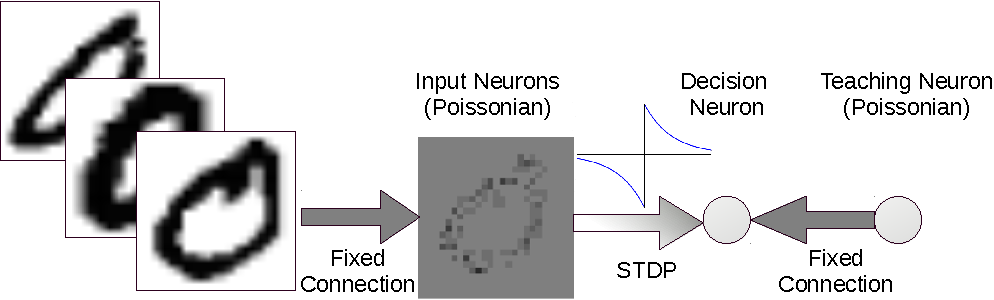
\includegraphics[width=0.48\textwidth]{images/training.pdf}
		} \\

	\centering
	
	\subfloat[Testing model of the spiking neural network.]{
		\label{Fig:test}
		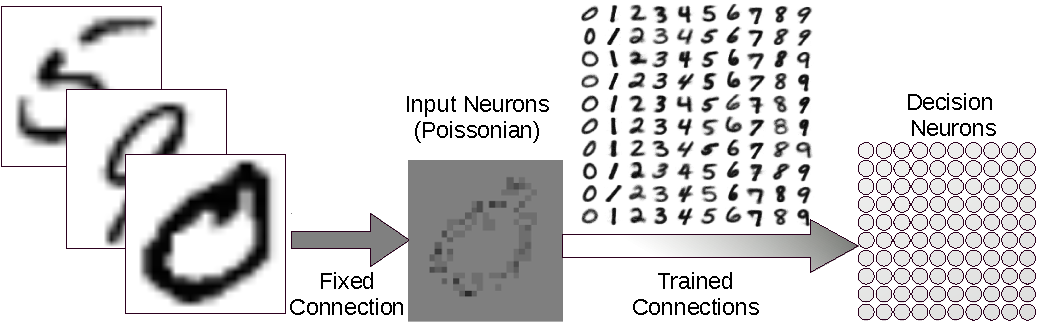
\includegraphics[width=0.48\textwidth]{images/testing.pdf}
		}
		
	\caption{The training and testing model of the two-layered spiking neural network.}
	\label{fig:model}
\end{figure} 



Both the training and testing exploited the Poissonian subset of the NE15-MNIST dataset.
Because different simulators generate random Poissonian spike trains with various mechanisms, languages and codes, using the same dataset is able to evaluate performance of these simulators without the interference by the non-unified input.
In terms of this case study, the performance of the model was evaluated with both software simulation (on NEST~[\cite{gewaltig2007nest}]) and hardware implementation (on SpiNNaker). 

%\subsection{Description of the data used}
\subsubsection{Training}

There are two layers in the neural network model.
And 28$\times$28 input neurons fully connected to 100 output neurons.
Each output neuron represented a trained template of a digit.
Thus there were 10 templates for each digit.
The firing rate of the input neurons were assigned linearly according to their intensities and normalised with a total firing rate of 2000~$Hz$.
The training set of 60000 hand written digits were firstly classified into 100 classes, 10 classes per digit, using K-means clusters.
Every image was presented 300~$ms$ during training and at the same time a teaching signal of 50~$Hz$ was conveyed to the responding output neuron (1 out of 100) to trigger the learning, see Fig~\ref{Fig:train}.
The trained weights were plotted in align with the input image size in Fig~\ref{Fig:test}.
%\begin{figure}[hbt!]
%	\centering
%	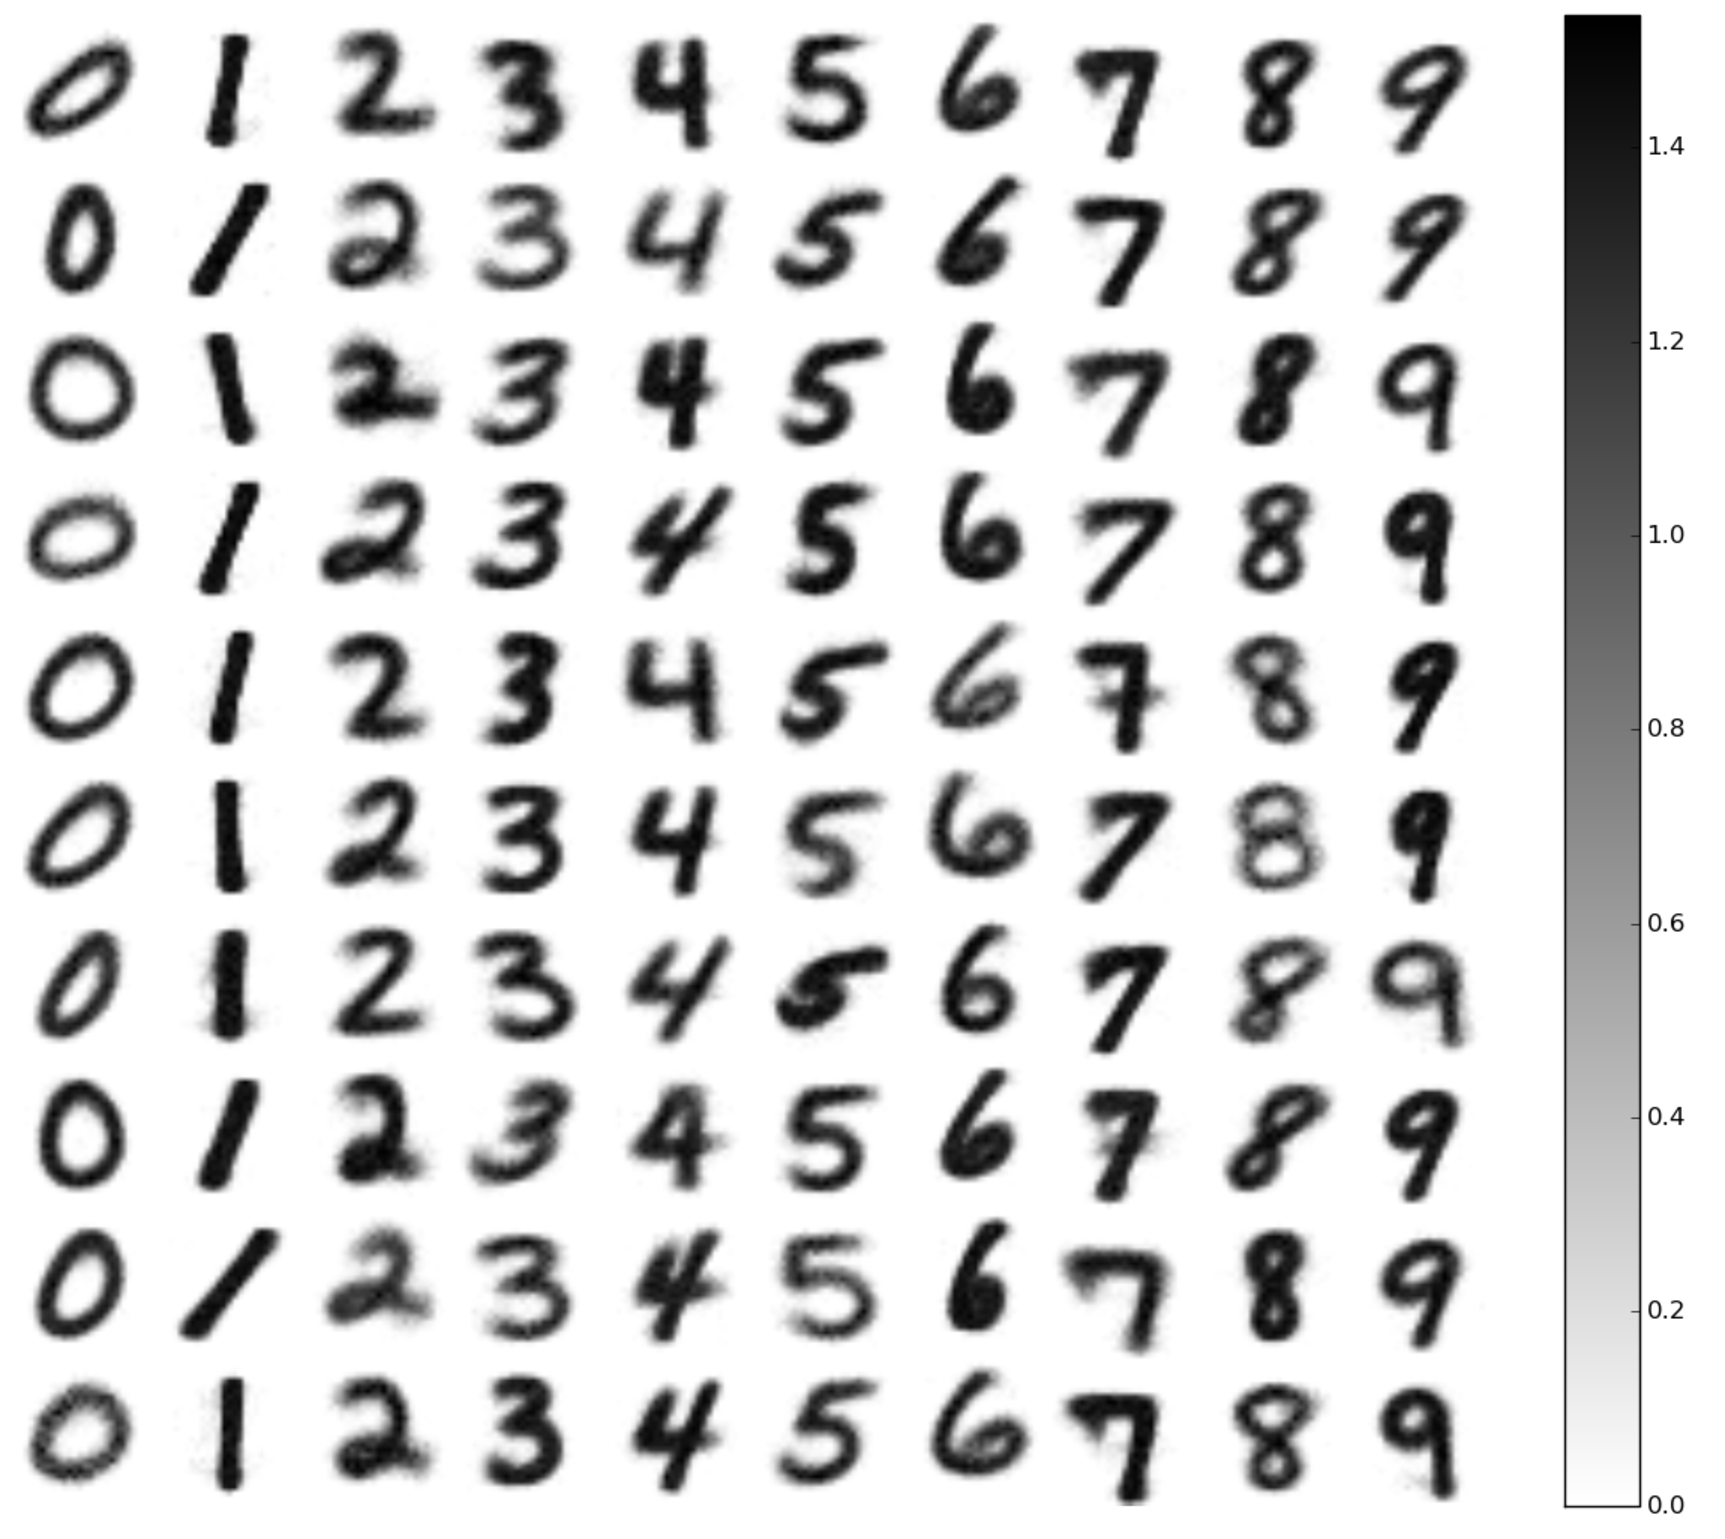
\includegraphics[width=0.48\textwidth]{images/weight_r.pdf}
%	\caption{Trained weights of the synapses from input layer to output neurons.}
%	\label{Fig:weight}
%\end{figure}  



\subsubsection{Testing}
The weights were normalised after training and applied to the same network.
And weak weights (=0) were set to inhibitory connections with an identical strength.
%The output neurons inhibited all the other neurons as a winner take all circuit.
The feed=forward testing network is shown in Fig~\ref{Fig:test}.
Poissonion spike trains are generated with input neurons and conveyed through trained synaptic connections to the decision neurons.
Every testing image was presented 1 second to the network, and the output neuron with the highest firing rate decides.
The accuracy of the recognition reached 82.42\%.%83.14\%.
The recording of the output neurons of a test sequence of digits (4, 1, 1, 0, 9, 3, 1, 9, 4, 6) was shown in the raster plot (Fig~\ref{Fig:output}).
Fig~\ref{Fig:test}.

\begin{figure}[hbt!]
	\centering
	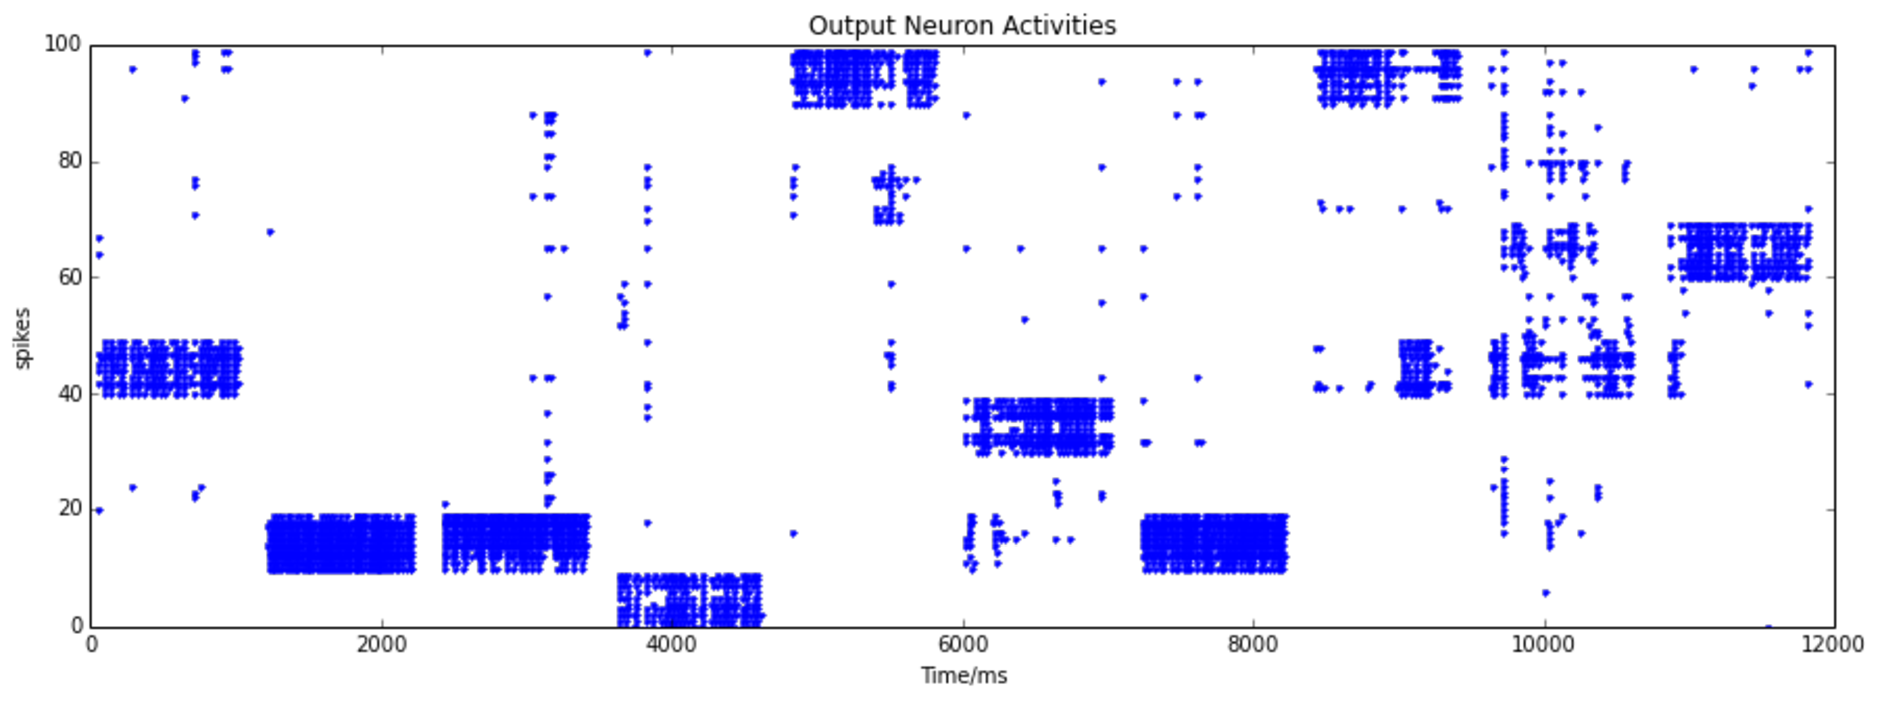
\includegraphics[width=0.48\textwidth]{images/test300-301.pdf}
	\caption{A raster plot of test of a digits sequence.}
	\label{Fig:output}
\end{figure} 
\subsubsection{Evaluation}

\subsection{[Evangelos Stromatias]Case Study II}
\textit{I will use the spiking DBN with the 7 hidden layers, 9 in total. It scores 97\%.}
\subsubsection{Training}
\subsubsection{Testing}
\subsubsection{Evaluation}

\begin{figure}[hbt!]
	\centering
	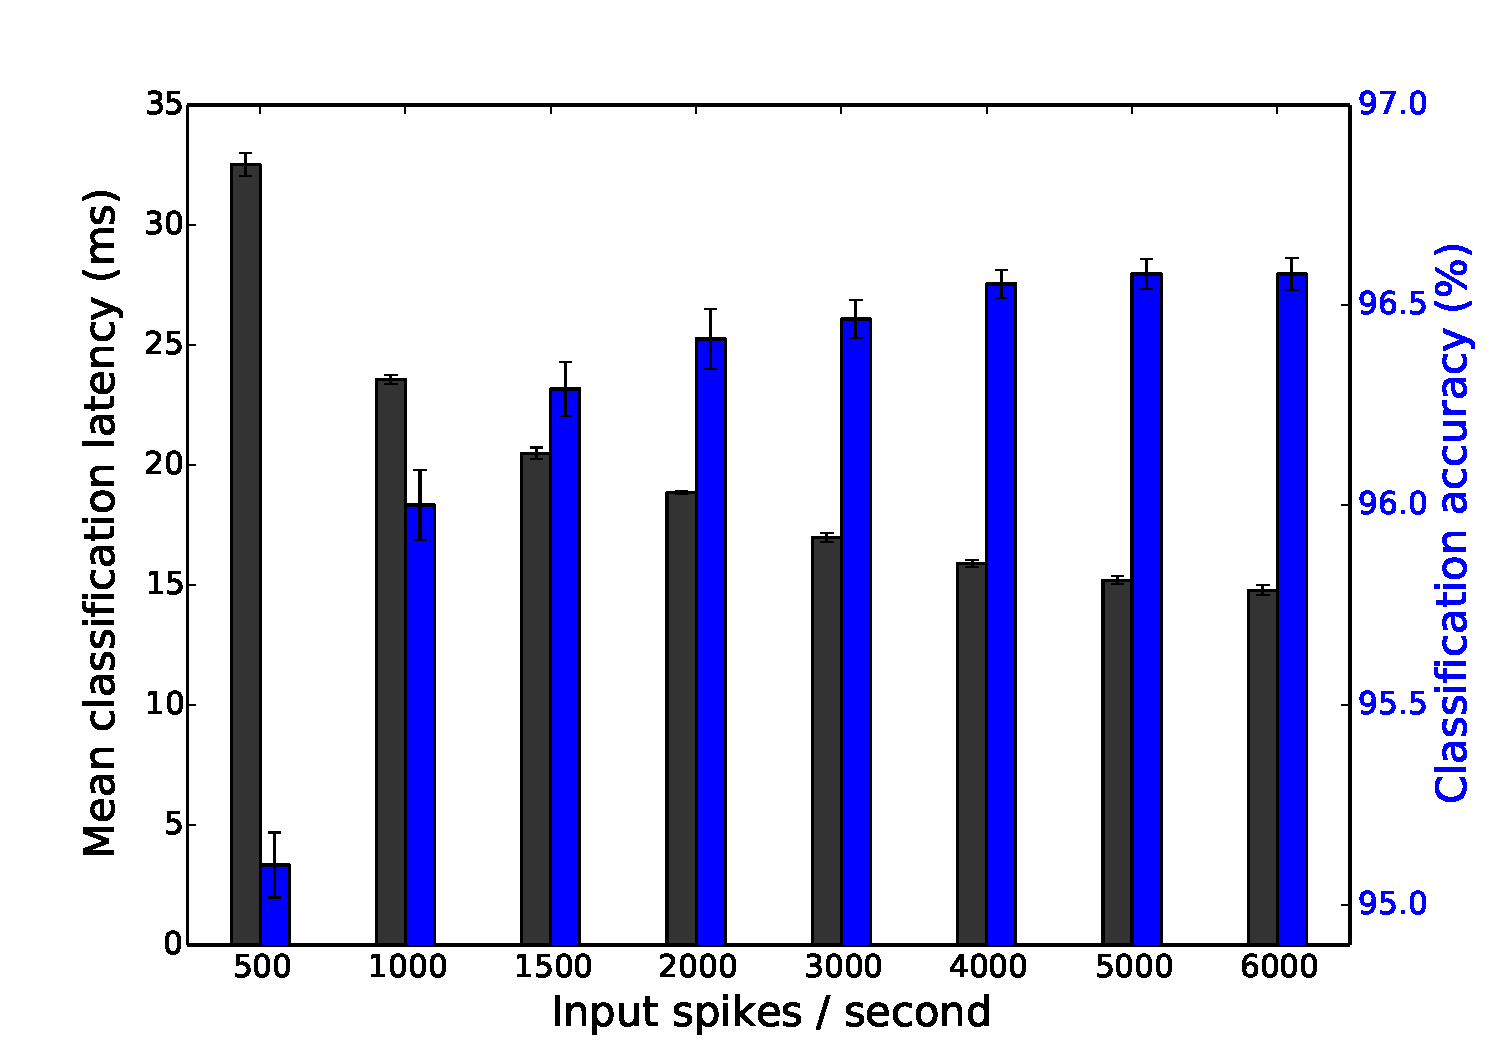
\includegraphics[width=0.48\textwidth]{images/evan/meanCAvsLatencyvsFiringrate_7hlayer.pdf}
	\caption{Classification accuracy as a function of the input firing rates.}
	\label{Fig:rateVSca}
\end{figure} 

\section{Conclusion}
\label{sec:summ}
\subsection{What we have said and done}
%The Proposal: Advantages
%In this work we propose a set of image conversion methods, in particular we have performed a full conversion of the MNIST database. Our implementations are open-source and can be obtained from a public repository.
%
%In order to ease the understanding and comparison of investigation results, we suggest that researchers report typical neural networks characteristics as well as others that we believe are important (e.g. events per time unit, time per sample, response time).
%
%The use of neuromorphic hardware in research is increasing, some of its characteristics may alter simulation results. We invite researchers to describe some hardware characteristics that have a direct implication in the performance of neural networks.

This paper puts forward the NE dataset as a baseline for comparisons on vision based SNNs.
It contains converted spike representations of existing widely-used databases in the vision recognition field.
Since new problems will be introduced continuously before vision becomes a solved question, the dataset will evolve as research develops. 
The conversion methods transforming images and videos to spike trains will advance, The number of vision databases included will increase and the corresponding evaluation methodology will evolve as well.
The dataset aims to provide a unified spike-based vision database and complementary evaluation methodologies to assess the performance of various SNN algorithms.
%(1) promote meaningful comparison among algorithms in the field of neural computation, (2) allow comparison with conventional image recognition methods, (3) provide an assessment of the state of the art in spike-based visual recognition, and (4) help researchers identify future directions and advance the field.

The first launch of the dataset is published as NE15-MNIST, which contains four different spike presentations of the stationary hand-written digit database.
The Poissonian subset aims at benchmarking the existing rate-based recognition methods.
The rank-order-encoded subset, FoCal, encourages research into spatio-temporal algorithms on recognition applications using only small numbers of input spikes.
Fast recognition can be verified on the subset of DVS recorded flashing input, since merely 30~ms of useful spike trains are recorded for each image.
As a step forward, the continuous spike trains captured from the DVS recorded moving input can be a good test on mobile neuromorphic robots.

The complementary evaluation methodology is essential to assess both the model-level and hardware-level performances.
For a network model, its topology, neuron and synapse models, and training methods are major descriptions for any kind of neural networks, including SNNs.
While the recognition accuracy, network latency and also the biological-time taken for both training and testing are specific performance measurements of a spike-based model.
To build any SNN model on a hardware platform, its network size will be constrained by the scalability of the hardware. Neural and synaptic models are limited to the ones that are physically implemented, unless the hardware platform supports programmability.
The accuracy of the results (e.g. CA) are naturally affected by the precision of the variable representing the membrane potential and synaptic weights.
Any attempts to implement an on-line learning algorithm on neuromorphic hardware must be backed by synaptic plasticity support.
Running an identical SNN model on different neuromorphic hardware platforms can not only expose if any of the previously mentioned capacities are supported, but also benchmark their performance on simulation time and energy usage.

Using the Poissonian subset of the NE15-MNIST dataset, two benchmark systems were proposed. 
The models were described and their performance on accuracy, network latency, simulation time and energy usage were presented.
These example benchmarking systems provided a recommended way of using the dataset and evaluating system performance.
They provide a baseline for comparisons and encourage improved algorithms and models to make use of the dataset.

Although spike-based algorithms have not surpassed their non-spiking counterparts in terms of recognition accuracy, they have shown great performance in response time and energy efficiency.
The dataset makes the comparison of SNNs with conventional recognition methods possible by using converted spike presentations of the same vision databases.
As the dataset grows, it will allow new problems to be investigated by researchers, which should allow the identification of future directions and, in consequence, advance the field.

%\subsection{The future direction of a developing database}
\subsection{The future direction of an evolving database}
The database will expand by converting more popular vision datasets to spike representations.
As mentioned in Section~\ref{sec:intro}, face recognition has become a hot topic in SNN approaches, however there is no unified spike-based dataset to benchmark theses networks.
Thus, the next development step for our dataset is to include face recognition databases.
While viewing an image,  saccades direct high-acuity visual analysis to a particular object or a region of interest and useful information is gathered during the fixation of several saccades in a second.
It is possible to measure the scan path or trajectory of the eyeball and the trajectories showed particular interest in eyes, nose and mouth while viewing a human face~\citep{yarbus1967eye}.
Therefore, our plan is also to embed modulated trajectory information to direct the recording using DVS sensors to simulate human saccades.


%While the major stumbling crux of the computer object recognition systems lies in the invariance problem.
Each encounter of an object on the retina is completely unique, because of the illumination (lighting conditions), position (projection locations on the retina), scale (distances and sizes), pose (viewing angles), and clutter (visual contexts) variabilities.
But the brain recognises a huge number of objects rapidly and effortlessly even in cluttered and natural scenes.
In order to explore invariant object recognition, the dataset is going to include the NORB (NYU Object Recognition Benchmark) dataset~\citep{lecun2004learning}, which contains images of objects that are first photographed in ideal conditions and then moved and placed in front of natural scene images.

Action recognition will be the first problem of video processing to be introduced in the dataset.
The initial plan is to use the DVS retina to convert KTH and Weizmann benchmarks to spiking versions.
Meanwhile, providing a software DVS retina simulator to transform  frames into spike trains is also on the schedule.
By doing this, huge number of videos, such as in YouTube, can automatically be converted to spikes, therefore providing researchers more time to work on their own applications.



\section*{Acknowledgments}
The work presented in this paper is largely inspired on discussions carried out at the 2015 Workshops on Neuromorphic Cognition Engineering in CapoCaccia.
The authors would like to thank the organisers and the sponsors.
The SpiNNaker project is supported by the Engineering and Physical Science Research Council (EPSRC grant EP/4015740/1), the EU Flagship Human Brain Project (FP7-604102), and also by ARM and Silistix.
The authors thank the support of these sponsors and industrial partners.
\bibliographystyle{frontiersinSCNS&ENG} % for Science and Engineering articles
%\bibliographystyle{frontiersinMED} % for Medicine articles

\bibliography{ref,rank-ordered,hw-ind-eval,hw-dep-eval}

\end{document}